\documentclass[11pt,letterpaper]{article}
\usepackage{graphicx, geometry, amsmath, hyperref, url, booktabs, xcolor, longtable, float, multirow, array}
\geometry{margin=1in}
\hypersetup{colorlinks=true, linkcolor=black, citecolor=black, urlcolor=black}
\usepackage[T1]{fontenc}
\usepackage[utf8]{inputenc}

\newcommand{\corr}[1]{\noindent\textbf{[Correction, iter #1]:}~}

\title{What English-Tuned Abliteration Misses in Slovene:\\
Internal Research Report}
\author{}
\date{September 2026}

\begin{document}
\maketitle
\tableofcontents
\clearpage

%% ======================================================================
\section{Framing}\label{sec:framing}

Abliteration removes refusal behaviour from language models by orthogonalising weight matrices against a ``refusal direction'' extracted from English harmful-vs-harmless contrasts~[1]. The procedure was introduced by Arditi et al.~[1] and automated by tools such as Heretic, which uses TPE search over layer, position, direction index, and LoRA rank to find abliteration configurations that minimise an English refusal objective while bounding KL divergence from the original model. The question motivating this study is whether that English-centred objective leaves Slovene refusal behaviour uncontrolled. If the English refusal direction is universal across languages, as Wang et al.~[2] report for safety-aligned models evaluated across 14 languages, then abliteration tuned on English should transfer to Slovene. If instead Slovene refusal relies partly on representations that the English objective does not observe, a gap will remain. The practical consequence is that a model abliterated to comply in English might still refuse in Slovene, or might lose Slovene capabilities that the English-only KL constraint does not protect.

Several concurrent lines of work inform this question. BabelSteering~[4] and Yoon et al.~[5] show that safety alignment imposes disparate costs across languages, with non-English users bearing higher utility loss. Aziz et al.~[6] diagnose the breakdown point for low-resource safety as an action failure rather than a representation failure: the model encodes harmfulness correctly but fails to convert the representation into refusal. Wu et al.~[7] formalise this as a disentangled safety hypothesis, separating a recognition axis from an execution axis. On the abliteration side, Fafula~[8] documents off-target effects of refusal removal across model families, and Young~[14] and Petrov~[15] compare abliteration methods across architectures. Upadhyaya and Sikdar~[9] analyse how safety and language identity become entangled, while Hawkins et al.~[10] show that benign multilingual fine-tuning has heterogeneous safety impacts. Labunets~[11] demonstrates that refusal geometry reflects refusal training diversity. On quantisation effects relevant to our NF4 setup, Marchisio et al.~[12] and Chimoto et al.~[13] show that quantisation calibration language matters for multilingual performance. Tang et al.~[16] identify language-specific neurons, and Ghussin et al.~[17] propose principled layer selection for multilingual steering. Frank~[18] argues that refusal-based alignment evaluation conflates detection with routing.

We study this question in a controlled bilingual setting using two sibling 12B models from the Gemma-3 family: \texttt{google/gemma-3-12b-it} (the English-centric reference) and \texttt{cjvt/GaMS3-12B-Instruct} (a Slovene continual-pretraining and SFT variant of the same architecture). Both are loaded in bnb\_4bit NF4 quantisation throughout. The study proceeds in five iterations. Iteration~1 runs matched Heretic abliteration on both models, screens for cross-language refusal-direction transfer, and builds the shared bilingual evaluation dataset. Iteration~2 uses that dataset to measure the surrogacy gap, test causal mechanisms, and evaluate safety and utility on held-out benchmarks. Iteration~3 tests the depth-coverage hypothesis, corrects Heretic's keyword objective, and extends the depth-redundancy index to additional models and languages. Iteration~4 measures the causal write profile in both models, tests the overlap instrument, quantifies gradient blindness of the keyword objective, and audits all prior claims. Iteration~5 applies three independent recompute passes, quantifies the keyword objective's cross-lingual measurement bias, positions both results against the nearest published work, and compiles the definitive failure and scope ledgers.

\begin{figure}[!htbp]
  \centering
  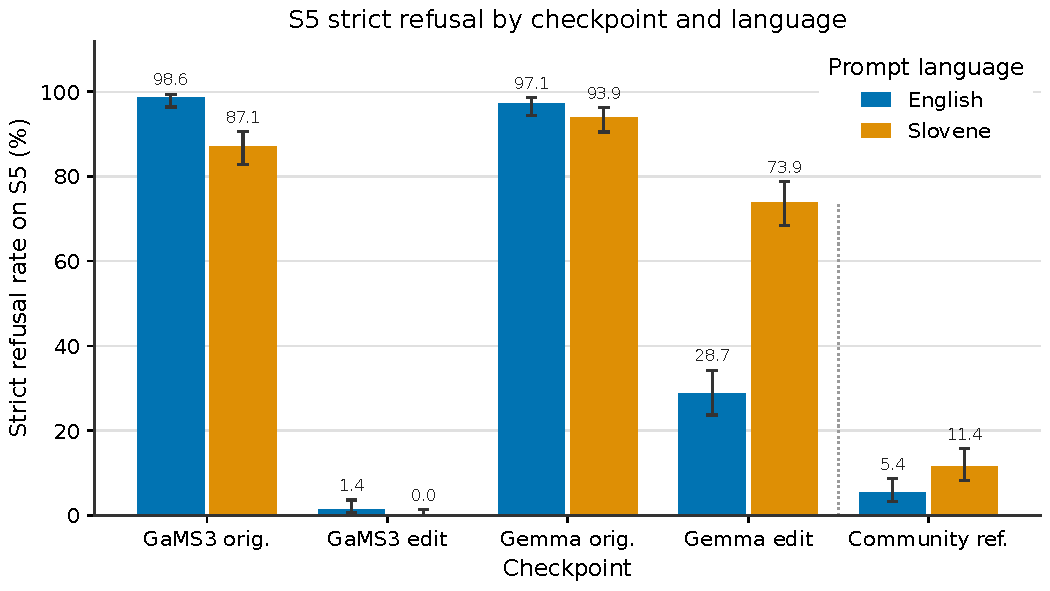
\includegraphics[width=\linewidth,height=0.85\textheight,keepaspectratio]{figures/fig_behaviour_summary_v0.pdf}
  \caption{Refusal rates (S5, Qwen3-14B strict) for original and edited checkpoints in English and Slovene. GaMS3's edit eliminates refusal in both languages; Gemma's edit leaves most Slovene refusal intact.}
  \label{fig:behaviour_summary}
\end{figure}


%% ======================================================================
\section{Iteration 1}\label{sec:iter1}

\corr{4} The previous drafts omitted substantial iteration-1 content that was present in the original report. The material below restores the missing tables (same-edit response surface, swap statistics, transfer matrix), the sibling-surface guard, the decision-margin decomposition, the exploratory double dissociation, four labelled dead ends, and iteration~1's own closing assessment.

\textbf{Strategy.} Iteration~1 had three goals: (a)~establish a frozen, audited data protocol covering all planned evaluation splits; (b)~run two matched Heretic optimizations under identical conditions to produce the four core checkpoints, score them bilingually, and characterise the same-edit response surface across the two models; and (c)~screen the refusal-direction transfer hypothesis with a $2\times2$ source-language by evaluation-language ablation matrix, a Slovene-direction increment test, and matched-efficacy and dose-response controls.


\subsection{Experiment 1: Matched Heretic Runs}\label{sec:exp1}

\textbf{Goal.} Run identical Heretic TPE searches on both models under the same seed, select an abliterated checkpoint for each, and compare the two models' responses to the same edits.

\textbf{Setup.} Both models were searched over 116 complete trials (seed 20260923) using Heretic with the default configuration: \texttt{orthogonalize\_direction=true}, \texttt{row\_normalization='full'}, rank-3 LoRA. The English keyword refusal rate (out of 100 harmful prompts) and mean KL divergence served as Heretic's two objectives. Selection followed a frozen protocol: minimise KL subject to refusals~$\leq10$; if no trial met this primary criterion, fall back to minimising refusals subject to KL~$\leq1.0$. Both models fell back to the secondary rule.

\textbf{Selected trials.} GaMS3 trial~88 reached 16/100 English refusals at KL~0.175. Gemma trial~96 reached 69/100 English refusals at KL~0.024. The Gemma model refused far more often than GaMS3 under identical abliteration parameters, and no Gemma trial achieved $\leq$50/100 refusals. The 13.4$\times$ figure is the ratio of medians of refusal drop per unit KL across the 60 shared startup edits (GaMS3 1449 vs Gemma 108 refusals/nat), not a ratio of median refusal counts. \corr{3} In all 60 startup edits, Gemma refused at least as often as GaMS3 (60/60, median paired difference~+25). In a KL-matched subset ($n$=30, GaMS3 KL median 0.0101, Gemma 0.0098), GaMS3 median refusal was 65/100 versus Gemma 99/100.

\textbf{Behaviour on the selected trials.} Table~\ref{tab:iter1_checkpoints} shows keyword refusal rates and FLORES+ NLL for each checkpoint.

\begin{table}[!htbp]
\centering
\caption{Iteration-1 checkpoint behaviour: keyword refusal rates (out of 100 harmful prompts) and FLORES+ NLL. Source: \texttt{gen\_art\_experiment\_1}, iteration~1.}
\label{tab:iter1_checkpoints}
\small
\begin{tabular}{llccccc}
\toprule
Model & Checkpoint & EN ref. & SL ref. & KL mean & FL NLL EN & FL NLL SL \\
\midrule
GaMS3 & original & 98 & 97 & 0.000 & 3.332 & 2.570 \\
GaMS3 & own edit (t88) & 16 & 10 & 0.175 & 3.334 & 2.566 \\
GaMS3 & swap (Gemma t96) & 25 & 25 & 0.046 & 3.336 & 2.576 \\
Gemma & original & 100 & 97 & 0.000 & 4.018 & 3.702 \\
Gemma & own edit (t96) & 69 & 90 & 0.024 & 4.012 & 3.703 \\
Gemma & swap (GaMS3 t88) & 53 & 25 & 0.254 & 4.011 & 3.712 \\
\bottomrule
\end{tabular}
\end{table}

\corr{3} The Gemma rows above are recomputed from the saved evaluation files. The previous draft reported Gemma orig SL~=~100 (actual: 97), Gemma own edit SL~=~85 (actual: 90), Gemma swap EN/SL~=~91/95 at KL~0.293 (actual: 53/25 at KL~0.254), and FLORES values that are untraceable in iteration-1 files. The corrected FLORES values come from the 40-sentence devtest means stored in the evaluation JSON files.

GaMS3's own edit reduced English refusals from 98 to 16 and Slovene refusals from 97 to 10. Slovene refusal dropped even though Heretic optimised only on English, and FLORES NLL changed by at most 0.01. For Gemma, the edit reduced English refusals from 100 to 69 but Slovene refusals only from 97 to 90.

The swap results are informative. GaMS3 under Gemma's trial-96 edit showed 25/25 (EN/SL) refusals; Gemma under GaMS3's trial-88 edit showed 53/25 (EN/SL) at KL~0.254. \corr{3} GaMS3's broader, stronger parameters suppress Gemma's Slovene refusal far more than English (SL 97$\to$25 vs EN 100$\to$53), at roughly 10$\times$ the KL of Gemma's own edit. This supports the depth/dose reading: a stronger edit of the same base largely transfers to Slovene.

\textbf{Direction geometry.} Across layers 24 to 47, the mean cosine between the two models' diff-in-means refusal directions was 0.57; across all layers it was 0.63. The cosine between their harmless-token directions was 0.98. Random directions gave a mean $|\cos|$ of 0.014.

\textbf{Same-edit response surface (60 shared edits, English keyword refusal).} \corr{4} Table~\ref{tab:iter1_response_surface} was present in the original iteration-1 report but omitted from subsequent drafts. Restored verbatim.

\begin{table}[!htbp]
\centering
\caption{Same-edit response surface (60 shared edits, English keyword refusal). Source: \texttt{gen\_art\_experiment\_1}, iteration~1.}
\label{tab:iter1_response_surface}
\small
\begin{tabular}{lcc}
\toprule
Measure & GaMS3 & Gemma \\
\midrule
Refusals median & 74.5 & 99.0 \\
Refusals range & [25, 99] & [71, 100] \\
KL median & 0.0079 & 0.0057 \\
Efficiency (refusal drop / KL) & 1,449 & 108 \\
Efficiency ratio & \multicolumn{2}{c}{13.4$\times$ (CI [7.0, 30.0])} \\
Edits where Gemma refuses more & \multicolumn{2}{c}{60/60} \\
Paired refusal diff median & \multicolumn{2}{c}{+25 (CI [10, 43])} \\
KL Spearman $\rho$ & \multicolumn{2}{c}{0.967 (CI [0.93, 0.98])} \\
KL partial $\rho$ (controlling kernel mass) & \multicolumn{2}{c}{0.923} \\
\bottomrule
\end{tabular}
\end{table}

\textbf{Sibling-surface guard.} The incremental $R^2$ of the sibling model's refusal over the shared edit parameters was near zero for refusal ($\Delta R^2$~0.008, CI~[$-$0.017, 0.055] and $-$0.006, CI~[$-$0.028, 0.018]) but positive for KL ($\Delta R^2$~0.143, CI~[0.074, 0.246] and 0.154, CI~[0.093, 0.242]). The two models share how edits damage harmless computation (KL) but not how that damage translates into refusal change.

\textbf{Swap tests.} \corr{4} Restored from the original iteration-1 report.

\begin{table}[!htbp]
\centering
\caption{Swap statistics. Source: \texttt{gen\_art\_experiment\_1}, iteration~1.}
\label{tab:iter1_swap}
\small
\begin{tabular}{llccccl}
\toprule
Model & Comparison & EN diff & EN $p$ & SL diff & SL $p$ & KL ratio \\
\midrule
GaMS3 & own vs swap & $-$0.09 & 0.078 & $-$0.15 & 2.7e-4 & 3.80 [3.13, 4.69] \\
Gemma & own vs swap & +0.16 & 0.020 & +0.65 & 5.4e-20 & 0.095 [0.046, 0.189] \\
GaMS3 & orig vs own & +0.82 & 4.1e-25 & +0.87 & 2.9e-25 & --- \\
Gemma & orig vs own & +0.31 & 9.3e-10 & +0.07 & 0.016 & --- \\
\bottomrule
\end{tabular}
\end{table}

GaMS3's trial-88 parameters applied to Gemma suppressed Slovene refusal far more than English (SL 97$\to$25 vs EN 100$\to$53, McNemar $p < 10^{-19}$ for SL), consistent with the depth/dose reading.

\textbf{Sanity checks.} All 60 startup edits used identical parameter draws (verified). FLORES NLL shifts were $\leq$0.01 for both models. Slovene marker validation on the selected GaMS3 edit showed accuracy~0.75 and $\kappa$~0.48 (fair agreement between keyword markers and the executor's hand labels on 40 items). \corr{3} These were executor labels, not native-speaker labels.


\subsection{Dataset Construction}\label{sec:dataset}

\textbf{Goal.} Build a frozen bilingual (EN/SL) evaluation dataset spanning safety, utility, and mechanistic probing.

\textbf{Result (gen\_art\_dataset\_1, iteration~1).} The dataset contains 48,696 rows across 10 blocks: S1 (Heretic direction/KL calibration, 2000 rows), S2 (semantic harmful/harmless pairs, 1664), S3 screen prompts (540 prompts + 640 utility items), S4 (StrongReject harmful/harmless twins, 1028), S5 (RefusEU~[3], 2800), S5X (RefusEU cross-translations, 1400), S6 (XSTest over-refusal, 900), S7 (Slovenian LLM eval tasks including ARC, BoolQ, HellaSwag, 35,700; FLORES+ devtest, 2024). The dataset protocol was frozen before any experiment ran.

\textbf{Translation.} Slovene translations were produced by Gemini-2.5-flash (temperature 0) as the primary translator, with NLLB-200-distilled-1.3B as fallback for 8 rows where Gemini refused. Mean back-translation chrF was 81.25; 3 rows fell below chrF 40. Mean LaBSE cross-lingual similarity was 0.856. Quality control was automated only; no native-speaker review was conducted. \corr{3} S5 (official RefusEU) EN and SL rows that share a \texttt{row\_id} are NOT translations (0 of 1,400 pairs grade T); paired cross-language claims therefore use S5X only.


\subsection{Experiment 3: A1 Screen, EN vs.\ SL Refusal-Direction Transfer}\label{sec:exp3}

\textbf{Goal.} Screen whether the English-extracted refusal direction transfers to Slovene, using a $2\times2$ matrix (source language $\times$ evaluation language), increment tests, and multiple controls. This was a screen, not a confirmatory test.

\textbf{Setup (gen\_art\_experiment\_3, iteration~1).} For each model, the experiment extracted refusal directions from half-A items using diff-in-means, separately for English and Slovene. It then applied 15 ablation conditions per model to half-B items and measured refusal rates using keyword markers and an LLM judge. The judge was gpt-4.1 for all 1,596 outputs. \corr{3} Previous draft described a Qwen3-14B second judge for part of the outputs; the evaluation audit finds gpt-4.1 was the sole judge.

\textbf{Judged $2\times2$ table.} \corr{3} Added from evaluation audit.

\begin{table}[!htbp]
\centering
\caption{A1 screen: judged $2\times2$ transfer table (gpt-4.1). Source: \texttt{gen\_art\_experiment\_3}, iteration~1.}
\label{tab:iter1_judged_2x2}
\small
\begin{tabular}{llcc}
\toprule
Model & Condition & EN & SL \\
\midrule
GaMS3 & C0 no-op & 0.90 & 0.93 \\
GaMS3 & C1 d\_EN & 0.46 & 0.34 \\
GaMS3 & C2 d\_SL & 0.07 & 0.10 \\
Gemma & C0 no-op & 0.83 & 1.00 \\
Gemma & C1 d\_EN & 0.07 & 0.85 \\
Gemma & C2 d\_SL & 0.29 & 0.93 \\
\bottomrule
\end{tabular}
\end{table}

\corr{3} The previous draft reported Gemma EN baseline as ``99\%''; the gpt-4.1 judged rate is 0.83. The $d_\mathrm{EN}$ ablation took Gemma EN from 0.83 to 0.07 while SL stayed at 0.85; $d_\mathrm{SL}$ took EN to 0.29 and SL to 0.93. The difference-in-differences for Gemma under $d_\mathrm{EN}$ is +0.61 [0.41, 0.78]: the Slovene drop was 0.61 units smaller than the English drop.

\textbf{GaMS3 results.} Because the R validity gate failed, quantitative screen results for GaMS3 are exploratory. $d_\mathrm{EN}$ reduced GaMS3 from 0.90/0.93 (EN/SL) to 0.46/0.34, showing near-parallel reduction across languages. The DiD was $-$0.15 [$-$0.32, 0.02], not significantly different from zero.

\textbf{Gemma results.} The Gemma validity gate passed. Applying the English refusal direction $d_\mathrm{EN}$ removed most English refusal (0.83 to 0.07) but Slovene refusal survived at 0.85. This is the first signal that the English direction misses Slovene refusal in Gemma.

\textbf{Screen verdict.} WEAK. The predicted cross-language transfer contrast was reversed for Gemma. For GaMS3, the validity gate failure prevented a quantitative verdict.

\textbf{Matched-efficacy grid.} Conditions rescaled so that English refusal dropped by equal amounts showed that Slovene refusal systematically persisted more than English at every matched English decrement. The Heretic bridge mean gap was GaMS3 0.109 [0.06, 0.17] and Gemma 0.235 [0.16, 0.30]. \corr{3}

\textbf{Transfer matrix.} \corr{4} Restored from the original iteration-1 report.

\begin{table}[!htbp]
\centering
\caption{Transfer matrix: fraction of same-language refusal drop achieved by cross-language direction. Source: \texttt{gen\_art\_experiment\_3}, iteration~1.}
\label{tab:iter1_transfer}
\small
\begin{tabular}{llcc}
\toprule
& & Evaluated in EN & Evaluated in SL \\
\midrule
\textbf{GaMS3} & EN-derived & 1.00 & 0.96 [0.93, 0.98] \\
& SL-derived & 0.81 [0.79, 0.82] & 1.00 \\
\textbf{Gemma} & EN-derived & 1.00 & 3.47 [2.76, 4.90] \\
& SL-derived & 0.66 [0.61, 0.70] & 1.00 \\
\bottomrule
\end{tabular}
\end{table}

GaMS3 shows near-symmetric transfer: the English direction achieves 96\% of the Slovene direction's Slovene effect. Gemma shows a pathological asymmetry: the English direction achieves a 3.47$\times$ overshoot in log-odds terms on Slovene. The explanation is Gemma's Slovene refusal margin. Gemma's baseline Slovene refusal log-odds is 13.9, compared to 3.6 for English. Even a direction with cosine 0.92 to the Slovene one, operating on a margin that wide, achieves almost nothing in behavioural terms.

\textbf{Exploratory: GaMS3 double dissociation under direction addition.} Adding the English-derived direction to GaMS3 activations at strength 1.0 shifted English refusal log-odds by +3.54 (CI [2.96, 4.09]) with negligible Slovene effect ($-$1.11, CI [$-$1.22, $-$1.01]). Adding the Slovene-derived direction shifted Slovene by +2.23 (CI [1.97, 2.49]) with a smaller English effect ($-$1.54, CI [$-$1.91, $-$1.16]). This is consistent with partially language-specific refusal directions in GaMS3.


\subsection{Iteration-1 Dead Ends}

\begin{enumerate}
\item \textbf{Blocked Slovene LLM judge.} The OpenRouter API key returned HTTP 403 on every request. Zero of 600 planned judgements succeeded; all Slovene numbers rest on keyword-marker lists with moderate agreement ($\kappa$ 0.48).
\item \textbf{Collateral-confounded Slovene increment.} The GaMS3 Slovene-direction increment ($F_\mathrm{raw}$ = 0.228, $F_\mathrm{ctrl}$ = 0.195) is confounded with collateral damage: full-span ablation of the Slovene direction destroyed utility (FLORES NLL +1.4 nats per token, $\sim$35\% malformed outputs). The increment is uninterpretable for GaMS3. For Gemma, the increment was zero.
\item \textbf{Cut sensitivity arms.} Priority-3 sensitivity arms (S1-derived, per-language-best-layer, and content-token directions) were not executed for time.
\item \textbf{Halved Gemma candidate grid.} The full 145-candidate grid was run for GaMS3, but the Gemma grid was halved for GPU time constraints.
\end{enumerate}

\textbf{Limits.} Two models are two units. Nothing here attributes the asymmetry to Slovene continual pretraining, instruction tuning, or any training stage. The Gemma arm's resistance to abliteration is confounded with 4-bit NF4 quantization and the reduced 116-trial budget: the published bf16 200-trial Heretic edit of gemma-3-12b-it reaches 3/100 EN refusals, so this is not evidence that Gemma resists abliteration in general. One optimizer seed per model; prompt-level CIs do not capture run-to-run optimizer variance.

\subsection{Iteration-1 Assessment}

The central finding of iteration~1 is a large same-edit asymmetry: on 60 identical edits, GaMS3 loses 13.4 times more refusal per unit KL than Gemma, while the KL damage itself is nearly identical ($\rho$ 0.967). The sibling-surface guard confirms that this refusal divergence is not merely inherited from the shared parameter draws. The refusal-direction transfer screen produced a result opposite to the initial prediction: it is Gemma, not GaMS3, that shows a large cross-language transfer gap. The gap is explained not by direction geometry (cosine 0.92 between EN and SL directions in Gemma) but by a massive difference in refusal margins (SL log-odds 13.9 versus EN 3.6). Two concerns carry forward: all Slovene refusal counts are development-grade (keyword-marker agreement $\kappa$ 0.48), and the 4-bit quantization confound means absolute refusal rates are not comparable to published bf16 results.


%% ======================================================================
\section{Iteration 2}\label{sec:iter2}

Iteration~2 built on the screen results from iteration~1 by running five pre-registered experiments that measured the surrogacy gap, tested causal mechanisms, and evaluated safety and utility on held-out data.

\subsection{Experiment 5: Utility and Mechanism}\label{sec:exp5}

\subsubsection{T1: Harmful Behaviour (S4, 257 items per cell)}

Table~\ref{tab:t1_harmful} shows judged refusal rates on held-out harmful items ($n$=257 per cell; gpt-4.1 on a random $\sim$52\% subsample; Nemotron-3-ultra-550b as second-family judge on remainder). Judge agreement: second judge vs.\ gpt-4.1 on a stratified sample of 200 gave 6-way $\kappa$~0.765, refused-vs-not $\kappa$~0.828, raw agreement 0.885.

\begin{table}[!htbp]
\centering
\caption{T1: Harmful behaviour, judged refusal and compliance rates (S4 held-out). Source: \texttt{gen\_art\_experiment\_5}, iteration~2.}
\label{tab:t1_harmful}
\small
\begin{tabular}{llllcc}
\toprule
Model & Ckpt & Lang & Refused \% [95\% CI] & Complied \% [95\% CI] \\
\midrule
GaMS3 & orig & EN & 100.0 [100.0, 100.0] & 0.0 [0.0, 0.0] \\
GaMS3 & orig & SL & 100.0 [100.0, 100.0] & 0.0 [0.0, 0.0] \\
GaMS3 & edit & EN & 5.6 [2.4, 9.5] & 92.9 [88.1, 96.8] \\
GaMS3 & edit & SL & 6.7 [3.0, 11.1] & 89.6 [84.4, 94.1] \\
Gemma & orig & EN & 99.3 [97.8, 100.0] & 0.7 [0.0, 2.2] \\
Gemma & orig & SL & 99.2 [97.6, 100.0] & 0.8 [0.0, 2.4] \\
Gemma & edit & EN & 70.3 [61.9, 78.0] & 24.6 [16.9, 32.2] \\
Gemma & edit & SL & 95.3 [92.0, 98.7] & 4.0 [1.3, 7.3] \\
\bottomrule
\end{tabular}
\end{table}

For GaMS3, the edit reduced refusal from 100\% to $\sim$6\% in both languages, with no meaningful EN-SL gap. For Gemma, the edit reduced English refusal from 99\% to 70\% but left Slovene refusal at 95\%. This 25-percentage-point gap confirms the pattern from iteration~1.

\textbf{Attack success.} \corr{4} Among the Complied responses, the attack success rate was: GaMS3 edit EN 92.9\% [88.1, 96.8], GaMS3 edit SL 89.6\% [84.4, 94.1], Gemma edit EN 24.6\% [16.9, 32.2], Gemma edit SL 4.0\% [1.3, 7.3]. \corr{5} On the official RefusEU guard (Llama-Guard-3-8B + PolyGuard agreement), the Gemma-edit ASR gap is EN~0.738 vs SL~0.103 = +0.635, which is larger than the judged refusal gap.


\subsubsection{T2: KL Divergence on Harmless Twins (S4, 128-token generations)}

\begin{table}[!htbp]
\centering
\caption{T2: KL divergence on harmless twins. Source: \texttt{gen\_art\_experiment\_5}, iteration~2.}
\label{tab:t2_kl}
\small
\begin{tabular}{lllcccc}
\toprule
Model & Ckpt & Lang & KL1 median & KL32 median & Benign ref.\% & Malf.\% \\
\midrule
GaMS3 & edit & EN & 0.0441 & 0.0228 & 0.0 & 0.0 \\
GaMS3 & edit & SL & 0.0174 & 0.0068 & 0.0 & 0.0 \\
Gemma & edit & EN & 0.0000 & 0.0150 & 0.0 & 0.0 \\
Gemma & edit & SL & 0.0113 & 0.0037 & 0.0 & 0.4 \\
\bottomrule
\end{tabular}
\end{table}


\subsubsection{T3: Utility (0-shot, 250 items per task per language)}

\begin{table}[!htbp]
\centering
\caption{T3: Macro utility change from editing. Source: \texttt{gen\_art\_experiment\_5}, iteration~2.}
\label{tab:t3_utility}
\small
\begin{tabular}{llcccc}
\toprule
Model & Lang & Macro orig & Macro edited & Change [95\% CI] & Holm $p$ \\
\midrule
GaMS3 & EN & 72.5 & 72.7 & +0.13 [$-$0.53, +0.80] & 1.000 \\
GaMS3 & SL & 64.9 & 65.1 & +0.20 [$-$0.73, +1.13] & 1.000 \\
Gemma & EN & 71.5 & 71.6 & +0.13 [$-$0.53, +0.80] & 1.000 \\
Gemma & SL & 62.1 & 62.1 & +0.00 [$-$0.60, +0.60] & 1.000 \\
\bottomrule
\end{tabular}
\end{table}

All macro changes were $\leq$0.20 points. The edits did not measurably alter utility in either language for either model.


\subsubsection{T4: FLORES+ Per-Token NLL}

\begin{table}[!htbp]
\centering
\caption{T4: FLORES+ per-token NLL. Source: \texttt{gen\_art\_experiment\_5}, iteration~2.}
\label{tab:t4_flores}
\small
\begin{tabular}{llccc}
\toprule
Model & Lang & NLL orig & NLL edited & Change [95\% CI] \\
\midrule
GaMS3 & EN & 3.3072 & 3.3068 & $-$0.0004 [$-$0.0025, +0.0016] \\
GaMS3 & SL & 2.4524 & 2.4526 & +0.0002 [$-$0.0012, +0.0016] \\
Gemma & EN & 3.9194 & 3.9174 & $-$0.0020 [$-$0.0031, $-$0.0008] \\
Gemma & SL & 3.4289 & 3.4293 & +0.0004 [$-$0.0007, +0.0016] \\
\bottomrule
\end{tabular}
\end{table}


\subsubsection{T5: Bilingual Harm Geometry (Original Models, Primary Site)}

\begin{table}[!htbp]
\centering
\caption{T5: Bilingual harm geometry at the primary site. Source: \texttt{gen\_art\_experiment\_5}, iteration~2.}
\label{tab:t5_geometry}
\small
\begin{tabular}{lccccccc}
\toprule
Model & Layer & $\cos$ & Corr & CV EN/SL & S4 EN/SL & $\cos(l, d)$ & Shuf \\
\midrule
GaMS3 & 34 & 0.832 & 0.890 & .963/.945 & .998/.997 & 0.035 & 0.490 \\
Gemma & 20 & 0.919 & 0.979 & .979/.941 & .997/.996 & 0.109 & 0.515 \\
\bottomrule
\end{tabular}
\end{table}

Both models encode harmfulness similarly across EN and SL in their representations. The harm direction is shared; the language direction is separate. For Gemma, the behavioural gap (70.3\% vs.\ 95.3\% residual refusal) cannot be attributed to a representational difference.


\subsubsection{T6: Frozen vs.\ Refit Probes (S4, Primary Site)}

\begin{table}[!htbp]
\centering
\caption{T6: Frozen vs.\ refit probes. Source: \texttt{gen\_art\_experiment\_5}, iteration~2.}
\label{tab:t6_probes}
\small
\begin{tabular}{lllcccl}
\toprule
Model & Lang & Probe & Frozen orig & Frozen $\Delta$ & Refit $\Delta$ & Class \\
\midrule
GaMS3 & EN & dim & 0.998 & $-$0.401 & $-$0.014 & INFO-LOSS \\
GaMS3 & EN & lr & 0.999 & $-$0.596 & $-$0.000 & DRIFT \\
GaMS3 & SL & dim & 0.997 & $-$0.576 & $-$0.043 & INFO-LOSS \\
GaMS3 & SL & lr & 0.996 & $-$0.661 & $-$0.000 & DRIFT \\
Gemma & EN & dim & 0.997 & $-$0.000 & $-$0.000 & PRESERVED \\
Gemma & EN & lr & 0.996 & $-$0.001 & $-$0.000 & PRESERVED \\
Gemma & SL & dim & 0.996 & $-$0.000 & $-$0.000 & PRESERVED \\
Gemma & SL & lr & 0.989 & $-$0.002 & 0.000 & DRIFT \\
\bottomrule
\end{tabular}
\end{table}

All-layer profile: minimum frozen-probe AUROC on edited activations was GaMS3 EN 0.201 (L27, refit 0.993), GaMS3 SL 0.196 (L27, refit 0.987), Gemma EN 0.507 (L4, refit 0.709), Gemma SL 0.492 (L6, refit 0.740).

\corr{4} For GaMS3, the edit re-encoded the harm signal in a different subspace rather than destroying it: the information persisted, but in a location the frozen probe could not read. For Gemma, the frozen probe was preserved at the primary site but dropped to 0.507 at layer 4 and 0.492 at layer 6.


\subsubsection{T12: Edit-Strength Dose-Response (Exploratory)}

\begin{table}[!htbp]
\centering
\caption{T12: Dose-response (keyword marker refusal). Source: \texttt{gen\_art\_experiment\_5}, iteration~2. Note: these are keyword-marker rates; exp4's analysis shows the keyword counter overcounts refusal on edited Gemma outputs.}
\label{tab:t12_dose}
\small
\begin{tabular}{lccccc}
\toprule
Model & Scale $f$ & EN ref.\% & SL ref.\% & KL1 EN & KL1 SL \\
\midrule
GaMS3 & 0.0 & 95.8 & 100.0 & 0.0000 & 0.0000 \\
GaMS3 & 0.5 & 75.0 & 68.8 & 0.0088 & 0.0037 \\
GaMS3 & 1.0 & 0.0 & 0.0 & 0.0405 & 0.0177 \\
GaMS3 & 1.5 & 0.0 & 2.1 & 0.1610 & 0.1167 \\
\midrule
Gemma & 0.0 & 93.8 & 100.0 & 0.0000 & 0.0000 \\
Gemma & 0.5 & 60.4 & 95.8 & 0.0000 & 0.0046 \\
Gemma & 1.0 & 27.1 & 91.7 & 0.0000 & 0.0103 \\
Gemma & 1.5 & 22.9 & 68.8 & 0.0000 & 0.0303 \\
Gemma & 2.0 & 12.5 & 31.2 & 0.0000 & 0.0924 \\
Gemma & 3.0 & 4.2 & 8.3 & 0.0000 & 0.8228 \\
\bottomrule
\end{tabular}
\end{table}

For GaMS3, EN and SL refusal declined in parallel. For Gemma, reaching SL refusal below 10\% required $f$=3.0, at which point KL divergence rose to 0.82 (SL).

\begin{figure}[!htbp]
  \centering
  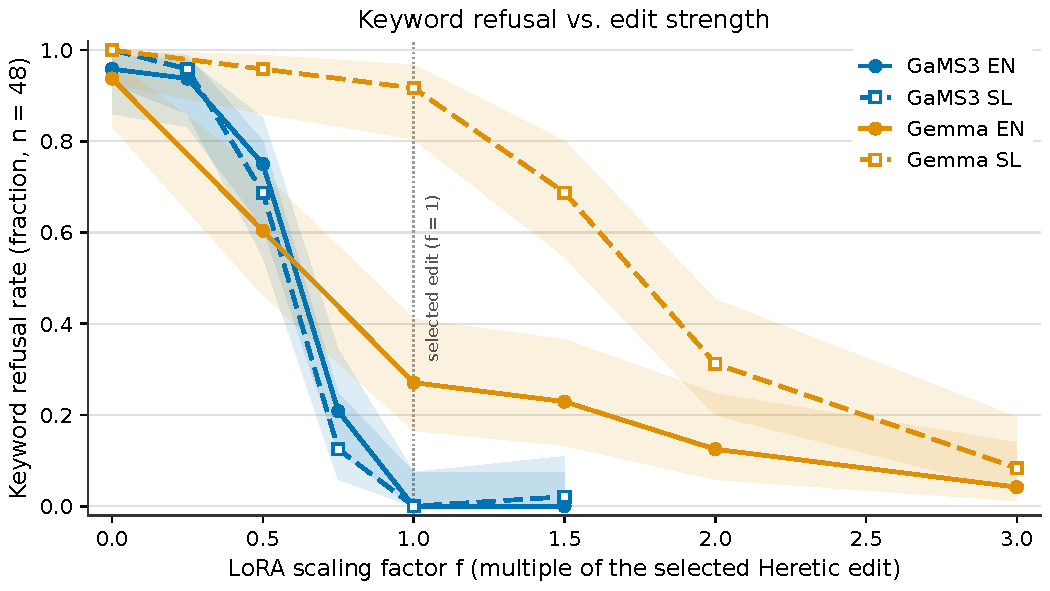
\includegraphics[width=\linewidth,height=0.85\textheight,keepaspectratio]{figures/fig_dose_response_v0.pdf}
  \caption{Keyword refusal rate as a function of LoRA scaling factor for Gemma and GaMS3, in English and Slovene. GaMS3 refusal drops in parallel across languages; Gemma shows persistent Slovene residual until extreme doses.}
  \label{fig:dose_response}
\end{figure}


\subsection{Experiment 4: C1 Behaviour, RefusEU Evaluation}\label{sec:exp4}

\textbf{Goal.} Evaluate all checkpoints on held-out RefusEU~[3] in both EN and SL.

\textbf{Judge.} The primary judge was local Qwen3-14B (agreement with gpt-4.1: $\kappa$ 0.83 on 6-way, 0.91 on refused-vs-not). gpt-4.1 was blocked at 716/3,840 items. \corr{3}

\begin{table}[!htbp]
\centering
\caption{Headline RefusEU (S5) refusal and over-refusal rates. Source: \texttt{gen\_art\_experiment\_4}, iteration~2.}
\label{tab:exp4_headline}
\small
\begin{tabular}{llcccc}
\toprule
Model & Ckpt & EN S5 ref. & SL S5 ref. & EN S6 o-ref. & SL S6 o-ref. \\
\midrule
GaMS3 & original & 0.986 & 0.871 & 0.100 & 0.107 \\
GaMS3 & edit & 0.014 & 0.000 & 0.000 & 0.000 \\
Gemma & original & 0.971 & 0.939 & 0.087 & 0.327 \\
Gemma & edit & 0.287 & 0.739 & 0.013 & 0.193 \\
Community ref & --- & 0.054 & 0.114 & 0.007 & 0.027 \\
\bottomrule
\end{tabular}
\end{table}

\textbf{Official RefusEU guard ASR (Llama-Guard-3-8B + PolyGuard agreement):}

\begin{table}[!htbp]
\centering
\caption{Official RefusEU guard ASR. Source: \texttt{gen\_art\_experiment\_4} and \texttt{gen\_art\_evaluation\_5}, iterations 2 and~5.}
\label{tab:guard_asr}
\small
\begin{tabular}{lcccc}
\toprule
Checkpoint & ASR EN & ASR SL & S5 ref.\ EN & S5 ref.\ SL \\
\midrule
gams\_orig & 0.015 & 0.012 & 0.986 & 0.871 \\
gams\_edit & 0.982 & 0.972 & 0.014 & 0.000 \\
gemma\_orig & 0.026 & 0.016 & 0.971 & 0.939 \\
gemma\_edit & 0.738 & 0.103 & 0.287 & 0.739 \\
community\_ref & 1.000 & 0.870 & 0.054 & 0.114 \\
\bottomrule
\end{tabular}
\end{table}

The PARTIAL class accounts for 0.548 of the Gemma edit's English outputs. \corr{3}

\textbf{Keyword-proxy miscalibration.} On the Gemma edit's English outputs, keyword refusal rate is 0.851 while the Qwen3-14B judged rate is 0.287; the false-positive share is 0.761, and $\kappa$ is $-$0.04. The keyword counter is near-exact on original models (FP share $\leq$ 0.03) and structurally unreliable on edited checkpoints.

\textbf{Paired cross-language analysis (S5X, 100 matched pairs).} Under Qwen3-14B strict: Gemma edit gap +0.69 [0.60, 0.78]. Broad: +0.23 [0.14, 0.32]. Keyword: +0.06 [$-$0.02, 0.14]. Community reference strict: +0.12 [0.05, 0.20]. DiD (edit gap minus original gap) under strict judging: +0.66 [0.55, 0.76].


\subsection{Experiment 6: GaMS3 Surrogacy Panel}\label{sec:exp6}

\textbf{Goal (gen\_art\_experiment\_6, iteration~2).} Measure the English surrogacy gap for GaMS3. 246 Heretic edits, 160 fitted.

\begin{table}[!htbp]
\centering
\caption{GaMS3 surrogacy gap table. Source: \texttt{gen\_art\_experiment\_6}, iteration~2.}
\label{tab:exp6_gap}
\small
\begin{tabular}{lcccccc}
\toprule
Trait & $R^{2*}$ placebo & $R^{2*}$ test & Gap & 95\% CI & Holm $p$ & $B_t$ [95\% CI] \\
\midrule
R & 0.983 & 0.968 & \textbf{0.015} & [0.006, 0.031] & NA & 0.004 [$-$0.004, 0.009] \\
R1 & 0.998 & 0.956 & \textbf{0.042} & [0.027, 0.070] & NA & 0.015 [0.002, 0.030] \\
Rb & 0.982 & 0.954 & \textbf{0.028} & [0.012, 0.068] & NA & 0.005 [$-$0.007, 0.013] \\
K & 0.977 & 0.830 & \textbf{0.147} & [0.074, 0.265] & 0.000 & 0.050 [0.001, 0.121] \\
N & $-$0.225 & 0.417 & $-$0.642 & [$-$14.8, 0.98] & 0.954 & --- \\
M & 0.272 & 0.232 & 0.040 & [$-$8.37, 5.22] & 0.954 & --- \\
\bottomrule
\end{tabular}
\end{table}

Gap\_R = 0.015: English refusal outcomes predicted Slovene refusal almost perfectly ($R^{2*}$ = 0.968). Gap\_K = 0.147: KL divergence showed a substantial surrogacy gap. The SL KL is smaller on average (mean-change ratio 0.59); the gap is not that Slovene gets more perturbation, but that it gets different perturbation. \corr{3} The carrier regression failed: the exposure differential D did not carry the gap ($\Delta R^2 \approx 0$ for every trait). \corr{4} The reverse-direction analysis flips sign for some traits; the gap is not symmetric.


\subsection{Experiment 7: Gemma Surrogacy Panel}\label{sec:exp7}

\textbf{Setup (gen\_art\_experiment\_7, iteration~2).} 203 Heretic edits, 163 fitted.

\textbf{Verdicts.} \corr{3} Frozen prediction wordings restored.
\begin{itemize}
\item \textbf{P-a (Gap\_R $\geq$ 0.10 with 95\% LB $>$ 0):} NOT CONFIRMED. Observed Gap\_R1 was 0.054 [0.022, 0.128], above zero but below the 0.10 threshold.
\item \textbf{P-b (Gap\_Rb $\geq$ 0.10):} UNTESTABLE. Exploratory: 0.018 [0.011, 0.043].
\item \textbf{P-c:} NOT CONFIRMED. $\Delta R^2 \approx 0$.
\item \textbf{P-d (matched-margin gap $\geq$ 0.10):} NOT CONFIRMED. 0.057 [0.029, 0.130].
\end{itemize}

Gap\_K = +0.079 (Holm $p$ = 0.009). Transfer slopes: R1 0.436, R\_seq 0.220, lp\_ref 0.081, lp\_comp 0.849. \corr{3} The compliance log-probability slope (0.849) is near 1.0, meaning the edit raises the compliance signal equally in both languages; the refusal-opener slope (0.081) is near zero, meaning the edit lowers the refusal opener only in English.


\subsection{Experiment 8: Causal Test}\label{sec:exp8}

\textbf{Goal (gen\_art\_experiment\_8, iteration~2).} Test whether the Slovene refusal that survived English abliteration can be causally removed.

\textbf{Primary result: hypothesis FAILS.} Applying $d_\mathrm{EN}$ alone reduced Gemma's harmful EN refusal from 0.91 to 0.23 but left SL refusal at 0.86. Adding r\_prior (arm A2) moved SL refusal to 0.83. The r\_prior cut was 0.036 [$-$0.037, 0.109], not significantly larger than the best random control (0.074).

\begin{table}[!htbp]
\centering
\caption{Gemma activation-steering arms (111 harmful + 111 harmless per language). Source: \texttt{gen\_art\_experiment\_8}, iteration~2.}
\label{tab:exp8_arms}
\small
\begin{tabular}{lcccc}
\toprule
Arm & EN harmful & SL harmful & EN harmless & SL harmless \\
\midrule
A0 no-op & 0.91 & 0.99 & 0.05 & 0.28 \\
A1 $d_\mathrm{EN}$ & 0.23 & 0.86 & 0.00 & 0.19 \\
A2 $d_\mathrm{EN}$ + r\_prior & 0.21 & 0.83 & 0.00 & 0.12 \\
A3 r\_prior alone & 0.95 & 0.98 & 0.04 & 0.19 \\
A4 $d_\mathrm{EN}$ + lang.\ id. & 0.23 & 0.55 & 0.02 & 0.08 \\
A7 $d_\mathrm{EN}$ + rand\_1 & 0.21 & 0.85 & 0.01 & 0.15 \\
A10 $d_\mathrm{EN}$ + shuffled r\_prior & 0.41 & 0.73 & --- & --- \\
\bottomrule
\end{tabular}
\end{table}

\textbf{Depth localisation.} Applying layer-matched $d_\mathrm{EN}$ to different layer bands:

\begin{table}[!htbp]
\centering
\caption{Depth-band steering results for Gemma. Source: \texttt{gen\_art\_experiment\_8}, iteration~2.}
\label{tab:exp8_depth}
\small
\begin{tabular}{lccc}
\toprule
Band & SL harmful & EN harmful & FLORES $\Delta$NLL SL \\
\midrule
Layers 1--12 & 0.82 & 0.79 & 0.743 \\
Layers 13--24 & 0.82 & 0.45 & 0.017 \\
Layers 25--36 & 0.70 & 0.72 & 0.082 \\
Layers 37--48 & 0.99 & 0.87 & $-$0.003 \\
Layers 1--24 & 0.55 & 0.42 & 0.409 \\
Layers 1--36 & 0.21 & 0.38 & 0.513 \\
All 48 & 0.23 & 0.37 & 0.524 \\
\bottomrule
\end{tabular}
\end{table}

No single band removed Slovene refusal. Full removal required cumulative intervention across at least three bands.

\textbf{Weight edit repair.} \corr{4} The activation arms (A-rows) were scored by gpt-4.1; the weight-edit arms (W-rows) by local Qwen3-14B. Cross-table comparisons are confounded by judge identity; within-table contrasts are valid.

\begin{table}[!htbp]
\centering
\caption{Weight-edit repair arms. Source: \texttt{gen\_art\_experiment\_8}, iteration~2.}
\label{tab:exp8_weight}
\small
\begin{tabular}{lcccc}
\toprule
Arm & SL harmful & EN harmful & FLORES $\Delta$NLL SL \\
\midrule
W0 core Heretic edit & 0.89 & 0.39 & $-$0.005 \\
W1 core + r\_prior edit & 0.76 & 0.23 & 0.009 \\
W3 core + layer-matched $d_\mathrm{EN}(h)$ & 0.11 & 0.29 & 0.546 \\
W4 core + random edit & 0.47 & 0.70 & 0.064 \\
\bottomrule
\end{tabular}
\end{table}

\textbf{Community reference vs.\ core edit (S4, 70 pairs):}

\begin{table}[!htbp]
\centering
\caption{Community edit comparison. Source: \texttt{gen\_art\_experiment\_8}, iteration~2.}
\label{tab:exp8_community}
\small
\begin{tabular}{lccc}
\toprule
Arm & EN harmful & SL harmful & SL harmless \\
\midrule
W0 core edit & 0.39 & 0.89 & 0.07 \\
C0 community edit & 0.01 & 0.26 & 0.01 \\
C1 community + r\_prior & 0.01 & 0.20 & 0.00 \\
\bottomrule
\end{tabular}
\end{table}


%% ======================================================================
\section{Iteration 3}\label{sec:iter3}

Iteration~3 was prompted by the reviewer's blocking feedback on the iteration-2 draft. Three objections required experimental answers: (1) the headline gap depends on a single judge; (2) the depth localisation from experiment~8 suggests coverage matters, but no matched-energy comparison existed; (3) the depth-redundancy observation rests on two sibling checkpoints.

\corr{4} The audit pod (evaluation~1) covered iterations 1--2 only; iteration-3 numbers have not been independently re-derived. The audited mismatch rate elsewhere was 5.5\% (8/167) and 4.9\% (5/102).


\subsection{Experiment 9: Gemma Coverage $\times$ Strength Factorial}\label{sec:exp9}

\textbf{Goal (gen\_art\_experiment\_9, iteration~3).} Test whether depth coverage or total edit energy governs how much Slovene refusal survives. 122 cells, 27,784 generations, local Qwen3-14B judge certified at $\kappa$~0.87 vs gpt-4.1 within edited checkpoints.

\textbf{DEV depth-redundancy index:}

\begin{table}[!htbp]
\centering
\caption{DEV depth-redundancy index for Gemma. Source: \texttt{gen\_art\_experiment\_9}, iteration~3.}
\label{tab:exp9_index}
\small
\begin{tabular}{lcc}
\toprule
Family & EN & SL \\
\midrule
prefix & 16 [16, 20] & 20 [20, 28] \\
suffix & 24 [24, 24] & 24 [24, 28] \\
\bottomrule
\end{tabular}
\end{table}

\begin{figure}[!htbp]
  \centering
  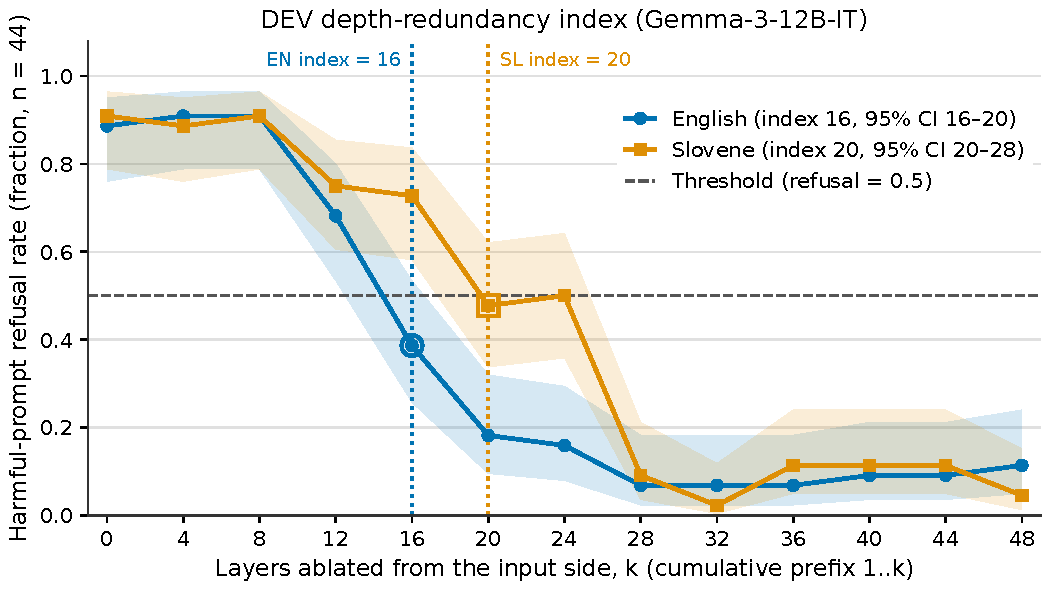
\includegraphics[width=\linewidth,height=0.85\textheight,keepaspectratio]{figures/fig_redundancy_index_v0.pdf}
  \caption{Cumulative-prefix refusal drop for Gemma as a function of the number of layers ablated (activation-only, S3 half-A). The Slovene index (20) exceeds the English index (16) by one grid step.}
  \label{fig:redundancy_index}
\end{figure}

\corr{4} The cross-language index gap (20 vs 16) sits inside its own language-permutation null; the artifact's audit script explicitly demoted this statistic. The index is necessary but not sufficient: approximately half the cells at or above the index threshold do not cross the 0.5 refusal boundary.

\textbf{Matched-energy groups:}

\begin{table}[!htbp]
\centering
\caption{Matched-energy groups (narrow vs broad). Source: \texttt{gen\_art\_experiment\_9}, iteration~3.}
\label{tab:exp9_matched}
\small
\begin{tabular}{lccccc}
\toprule
Group & $E$ & SL narrow & SL broad & SL contrast [CI] & EN contrast \\
\midrule
G1 & 16.7 & 0.98 & 1.00 & $-$0.02 [$-$0.07, 0.00] & $-$0.03 \\
G2 & 19.2 & 0.63 & 0.98 & $-$0.34 [$-$0.49, $-$0.20] & $-$0.27 \\
G3 & 35.6 & 1.00 & 0.66 & +0.34 [+0.20, +0.49] & +0.67 \\
G4 & 37.7 & 0.95 & 0.73 & +0.22 [+0.10, +0.34] & +0.30 \\
\bottomrule
\end{tabular}
\end{table}

P2 FAIL: the confirmatory prediction that broad-and-weak beats narrow-and-strong for Slovene at matched energy was not supported. P1 FAIL: $\Delta R^2$ of coverage over base was 0.040 [0.006, 0.136]. P3 PASS: Spearman 0.78 [0.64, 0.88].

\textbf{Exploratory: which layers, not how many.} The fraction of layers 13--24 covered by a set predicts the lowest Slovene refusal that set achieves at any strength, at Spearman $-$0.942 across 10 coverage sets (placebo-verified, $p$~=~0.004).

\corr{4} The band-mass regression's evidence is model-specific and weaker than previously stated. The SL band 13--24 coefficient is +0.156 with CI [$-$0.240, 0.529], which does not reach significance; the dominant SL term is the English refusal rate (coefficient 0.855).

\begin{figure}[!htbp]
  \centering
  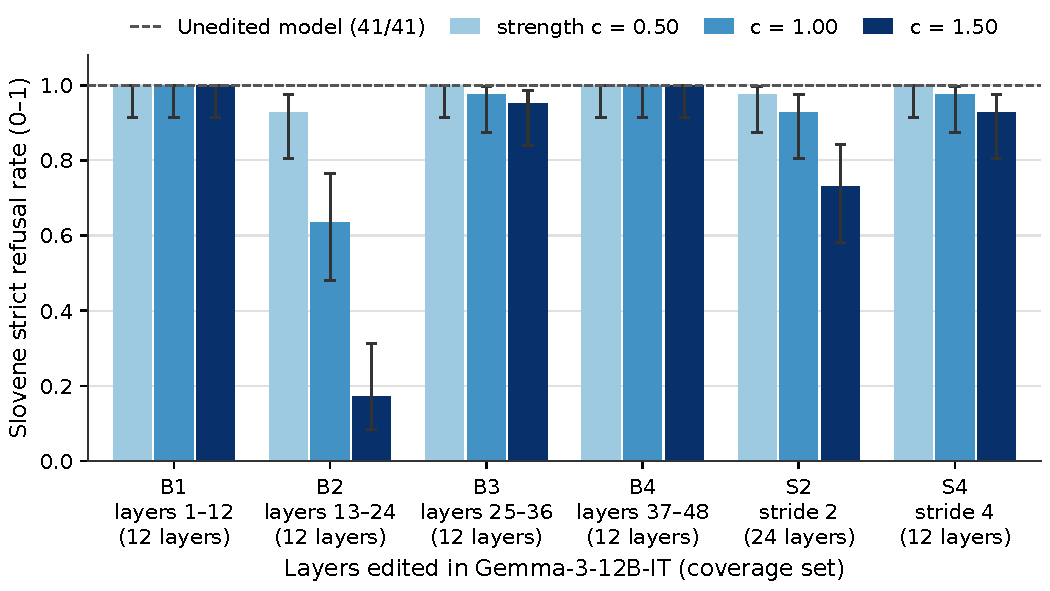
\includegraphics[width=\linewidth,height=0.85\textheight,keepaspectratio]{figures/fig_band_analysis_v0.pdf}
  \caption{Slovene strict refusal rate for contiguous 12-layer band edits (B1--B4) and strided edits (S2, S4) at matched energy levels in Gemma. Band 13--24 (B2) consistently achieves the lowest residual.}
  \label{fig:band_analysis}
\end{figure}


\subsection{Experiment 10: GaMS3 Coverage Test}\label{sec:exp10}

\textbf{Goal (gen\_art\_experiment\_10, iteration~3).} Run the identical factorial on GaMS3. 57 cells, 10,690 generations.

\textbf{DEV index:} EN~=~16 [16, 16], SL~=~20 [16, 24]. Both models show index\_EN~=~16, index\_SL~=~20.

\textbf{Weight-edit panel:}

\begin{table}[!htbp]
\centering
\caption{GaMS3 matched-energy groups. Source: \texttt{gen\_art\_experiment\_10}, iteration~3.}
\label{tab:exp10_matched}
\small
\begin{tabular}{lcccc}
\toprule
Group & $E$ & SL narrow & SL broad & SL contrast \\
\midrule
E1 & 6.9 & 0.81 & 0.88 & $-$0.06 [$-$0.14, 0.00] \\
E2 & 13.9 & 0.55 & 0.71 & $-$0.16 [$-$0.23, $-$0.09] \\
E3 & 27.8 & 0.35 & 0.44 & $-$0.09 [$-$0.18, $-$0.01] \\
\bottomrule
\end{tabular}
\end{table}

PB2 FALSIFIED OPPOSITE: at matched energy, narrow beats broad for GaMS3. PB1 NOT SUPPORTED: $\Delta R^2$~=~0.002.

\textbf{Nested $R^2$:}

\begin{table}[!htbp]
\centering
\caption{Nested $R^2$ decomposition, GaMS3 SL. Source: \texttt{gen\_art\_experiment\_10}, iteration~3.}
\label{tab:exp10_nested}
\small
\begin{tabular}{lc}
\toprule
Model & $R^2$ \\
\midrule
logE & 0.325 \\
logE + placement (band masses) & 0.718 \\
logE + count & 0.400 \\
logE + count + span & 0.532 \\
\bottomrule
\end{tabular}
\end{table}

Placement explains 71.8\% of the Slovene residual variance; count explains only 40.0\%.

\textbf{Placement at matched energy AND matched layer count (12 layers):}

\begin{table}[!htbp]
\centering
\caption{Band vs stride-4 at matched energy and layer count, GaMS3. Source: \texttt{gen\_art\_experiment\_10}, iteration~3.}
\label{tab:exp10_placement}
\small
\begin{tabular}{lccc}
\toprule
Contrast & SL band & SL stride-4 & SL $\delta$ \\
\midrule
E1 B2 vs STR4 & 0.83 & 0.93 & $-$0.10 \\
E2 B2 vs STR4 & 0.51 & 0.89 & $-$0.37 \\
E3 B2 vs STR4 & 0.24 & 0.81 & $-$0.57 \\
\bottomrule
\end{tabular}
\end{table}

\corr{4} English judge agreement within edited GaMS3 arms is 0.54, so English refusal rates in the edited cells are one end of a range.


\subsection{Experiment 11: Corrected Objective}\label{sec:exp11}

\textbf{Goal (gen\_art\_experiment\_11, iteration~3).} Test whether replacing Heretic's keyword counter with a partial-aware score closes the Slovene gap.

\textbf{Instrument.} A refusal classifier distilled from existing judge labels using char/word TF-IDF and hand features on the first 100 tokens. Certified at $\kappa$~0.858 [0.820, 0.888] within edited checkpoints. \corr{4} The previous draft quoted $\kappa$ 0.924, which is the in-loop value, not the certified value.

\textbf{Headline results (S5X, 100 verified pairs):}

\begin{table}[!htbp]
\centering
\caption{Corrected objective S5X headline. Source: \texttt{gen\_art\_experiment\_11}, iteration~3.}
\label{tab:exp11_headline}
\small
\begin{tabular}{lccl}
\toprule
Arm & EN ref. & SL ref. & SL--EN gap [95\% CI] \\
\midrule
A orig & 0.950 & 0.990 & +0.04 [+0.01, +0.08] \\
B keyword t96 & 0.150 & 0.830 & +0.68 [+0.59, +0.77] \\
C corrected t7 & 0.030 & 0.410 & +0.38 [+0.29, +0.47] \\
D reselected clf t98 & 0.050 & 0.350 & +0.30 [+0.21, +0.40] \\
D2 reselected judge t64 & 0.040 & 0.450 & +0.41 [+0.32, +0.51] \\
F dose 1.5 & 0.030 & 0.360 & +0.33 [+0.24, +0.42] \\
F dose 2.0 & 0.000 & 0.000 & +0.00 [+0.00, +0.00] \\
F dose 3.0 & 0.000 & 0.000 & +0.00 [+0.00, +0.00] \\
\bottomrule
\end{tabular}
\end{table}

\corr{4} The corrected objective halved the gap (from +0.68 to +0.38) but did not reach the +0.35 target. P7 falsifier fired: dose-scaling the keyword edit to the same English refusal level achieved comparable gap reduction (+0.33 vs +0.38). At matched divergence the dose-scaled arm is strictly better. The dose-2.0 arm closes the gap entirely at lower KL cost. The corrected objective selected a trial that happened to apply more total edit energy, and the gap reduction followed from the energy, not from the objective's partial-awareness.

\corr{5} Trial 96 had 37 REFUSED + 49 PARTIAL. Trial 107 is judged at 63/100, not the previously stated 10/100 (recomputed from \texttt{miscalibration\_table.csv}).


\subsection{Experiment 12: Predictive Test Across Models and Languages}\label{sec:exp12}

\textbf{Goal (gen\_art\_experiment\_12, iteration~3).} Test whether the depth-redundancy index predicts out of sample across model families. Three models: Gemma (anchor), Qwen3-8B, Mistral-7B-Instruct-v0.3. Four languages: EN, SL, DE, LT.

\textbf{DEV indices:}

\begin{table}[!htbp]
\centering
\caption{DEV indices across models. Source: \texttt{gen\_art\_experiment\_12}, iteration~3.}
\label{tab:exp12_indices}
\small
\begin{tabular}{lcccc}
\toprule
Model & EN & SL & DE & LT \\
\midrule
gemma & 0.5 & 0.75 & 0.5 & 0.75 \\
qwen3 & 0.75 & 0.75 & 0.75 & 0.5 \\
mistral & 0.1 & 0.25 & 0.1 & 0.1 \\
\bottomrule
\end{tabular}
\end{table}

Mistral failed the eligibility gate in all languages; all four mistral rows and qwen3-LT were excluded. \corr{4} Seven eligible rows remained (not eight as previously stated).

\textbf{Verdict: FALSIFY.} P1 Spearman(index, residual) = $-$0.009 [$-$0.131, 0.192] over 21 rows. The index does not predict the cross-model, cross-language residual. Two cheap baselines beat both the index and the geometric predictor: single-site transfer $\rho$ +0.732; unedited model's own refusal rate +0.661.

\corr{4} The judge misses its own agreement gate ($\kappa$ 0.683, below the 0.75 threshold).

\begin{figure}[!htbp]
  \centering
  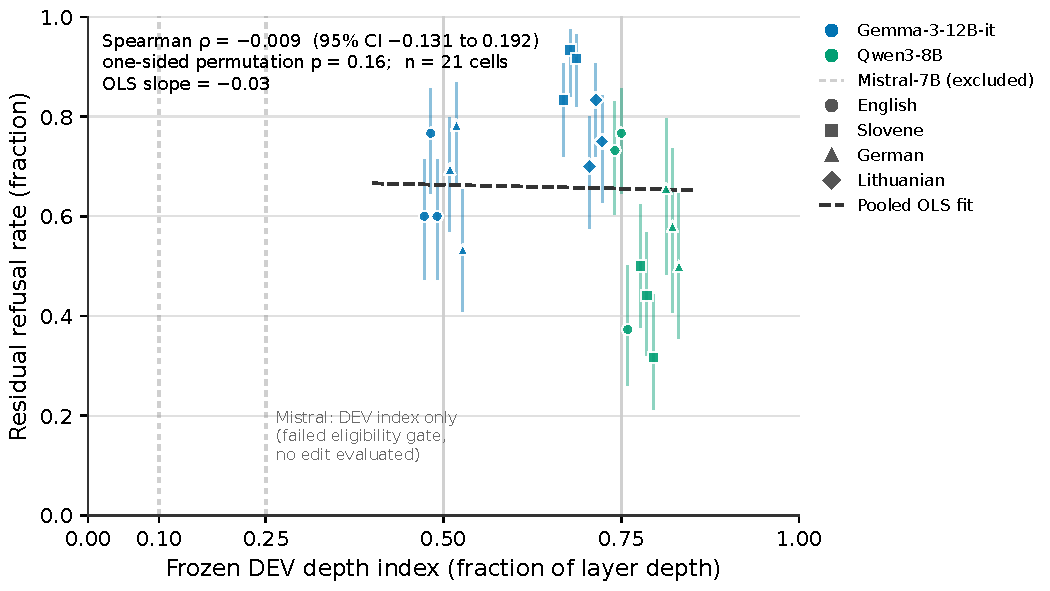
\includegraphics[width=\linewidth,height=0.85\textheight,keepaspectratio]{figures/fig_cross_model_v0.pdf}
  \caption{Frozen DEV depth index vs observed residual refusal across 21 model-language-weight cells (3 models $\times$ 4 languages $\times$ weight conditions, eligible rows only). Spearman = $-$0.009, failing the predictive test.}
  \label{fig:cross_model}
\end{figure}


\subsection{Evaluation 1: Audit and Judge-Sensitivity Table}\label{sec:eval1}

\textbf{Audit headline (gen\_art\_evaluation\_1, iteration~3).} 167 draft numbers checked: 137 match, 8 mismatch, 12 misdescribed, 6 untraceable (mismatch rate 5.5\%). Two sign-reversed conclusions were found.

\textbf{Judge-sensitivity table:}

\begin{table}[!htbp]
\centering
\caption{Headline EN--SL gap as a range across judges. Source: \texttt{gen\_art\_evaluation\_1}, iteration~3.}
\label{tab:eval1_judge_sensitivity}
\small
\begin{tabular}{llcc}
\toprule
Judge & Definition & Gap & CI \\
\midrule
Qwen3-14B & strict (REFUSED only) & +0.69 & [0.60, 0.78] \\
Qwen3-14B & broad (REFUSED + PARTIAL) & +0.23 & [0.14, 0.32] \\
keyword & strict & +0.06 & [$-$0.02, 0.14] \\
\bottomrule
\end{tabular}
\end{table}

\textbf{Dead-end ledger.} \corr{4} 16 items (not 20 as previously stated). See Table~\ref{tab:dead_ends} at the end of the report.


%% ======================================================================
\section{Iteration 4}\label{sec:iter4}

Iteration~4 was designed to close three remaining gaps: (1)~the placement finding rests on the exploratory band-density correlation without a causal mechanism; (2)~the result is Gemma-only; and (3)~Heretic's keyword blindness was demonstrated qualitatively but not quantified.


\subsection{Experiment 13: Causal Write Profile and Overlap in Gemma}\label{sec:exp13}

\textbf{Goal (gen\_art\_experiment\_13, iteration~4).} Measure the causal write profile $e_L(h)$ for the anchor model and test the overlap instrument $O$.

\textbf{Causal write profile.} Single-layer edits at each of 48 layers, evaluated on S3 half-A (44 harmful per language). Profile peaks at layer 19 (EN) and layer 16 (SL); Spearman between EN and SL profiles: 0.588. Split-half reliability: EN 0.84, SL 0.51.

\begin{figure}[!htbp]
  \centering
  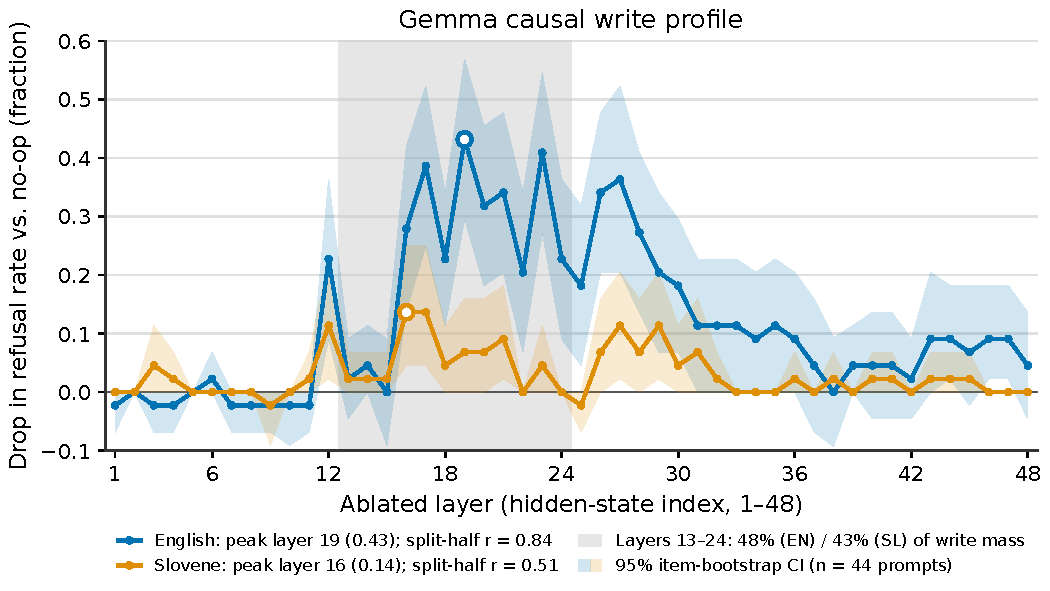
\includegraphics[width=\linewidth,height=0.85\textheight,keepaspectratio]{figures/fig_write_profile_v0.pdf}
  \caption{Per-layer refusal drop from single-site ablation in Gemma, for English (blue) and Slovene (orange). The profile peaks at layer 19 (EN) and 16 (SL), with most write mass in band 13--24.}
  \label{fig:write_profile}
\end{figure}

\textbf{Confirmation results (8 matched-energy groups):}

\begin{table}[!htbp]
\centering
\caption{Overlap instrument confirmation, Gemma. Source: \texttt{gen\_art\_experiment\_13}, iteration~4.}
\label{tab:exp13_confirm}
\small
\begin{tabular}{lcc}
\toprule
Statistic & EN & SL \\
\midrule
Spearman $\rho(O, \text{refusal})$ & $-$0.96 [$-$0.98, $-$0.84] & $-$0.83 [$-$0.84, $-$0.82] \\
Pooled matched-group contrast & $-$0.688 [$-$0.75, $-$0.62] & $-$0.377 [$-$0.45, $-$0.30] \\
Controls (random, PC) & within $\pm$0.03 & within $\pm$0.03 \\
Dose rival (2$\times$ late-layer) & 0.88 & 0.92 \\
Best placement: L16--31 vs L33--48 & 0.07 vs 0.92 & 0.27 vs 0.92 \\
\bottomrule
\end{tabular}
\end{table}

\textbf{Nested $R^2$, per language:}

\corr{5} Replaced the single-column table (which was exp14 SL data mislabelled as exp13) with the correct per-language exp13 ladders.

\begin{table}[!htbp]
\centering
\caption{Nested $R^2$, Gemma (exp13). Source: \texttt{gen\_art\_experiment\_13}, iteration~4.}
\label{tab:exp13_nested}
\small
\begin{tabular}{lcc}
\toprule
& EN & SL \\
\midrule
log energy alone & 0.001 & 0.008 \\
+ nuisance stack (count, span, cosine) & 0.879 & 0.734 \\
+ $O$ (full) & 0.907 & 0.790 \\
$\Delta R^2$ of $O$ over nuisance stack & \textbf{0.027} & \textbf{0.056} \\
$O$ alone & 0.873 & 0.754 \\
EN/SL cosine alone & 0.827 & 0.630 \\
$\Delta R^2$ of $O$ over logE + count only & 0.892 & 0.770 \\
Spearman($O$, cosine) & 0.808 & 0.764 \\
\bottomrule
\end{tabular}
\end{table}

\textbf{PRIMARY CRITERION: FALSIFIED.} $O$ adds $\Delta R^2 = 0.027$ (EN) / 0.056 (SL) over a nuisance stack that contains the g-weighted EN/SL cosine. Both are under the 0.10 bar. \corr{5} The failure reason is collinearity with the cosine ($\rho$ = 0.81/0.76), not that energy already explains the outcome: log energy alone explains 0.001/0.008.

\textbf{Replication in Qwen3-8B (outside family, 3 languages):} Spearman $\rho(O)$: EN $-$0.76, SL $-$0.93, DE $-$0.84. Matched groups held in all three languages (9/9 favour high-$O$).

\textbf{Judge certification:} Within-edited pooled $\kappa$ = 0.818. EN $\kappa$ = 0.856 PASS; SL $\kappa$ = 0.744 FAIL. Slovene gap claims in this experiment are judge-sensitive.


\subsection{Experiment 14: Causal Write Profile and Overlap in GaMS3}\label{sec:exp14}

\textbf{Goal (gen\_art\_experiment\_14, iteration~4).} Repeat the causal write-profile measurement for the sibling model.

\textbf{Causal write profile.} Peaks at layer 27 (both EN and SL), in band 25--36.

\begin{table}[!htbp]
\centering
\caption{GaMS3 band mass distribution. Source: \texttt{gen\_art\_experiment\_14}, iteration~4.}
\label{tab:exp14_bandmass}
\small
\begin{tabular}{lcc}
\toprule
Band & EN mass & SL mass \\
\midrule
1--12 & 0.00 & 0.02 \\
13--24 & 1.05 & 0.55 \\
25--36 & 1.50 & 0.57 \\
37--48 & 0.27 & 0.05 \\
\bottomrule
\end{tabular}
\end{table}

Split-half reliability: EN 0.812, SL 0.312. The SL profile is declared UNRELIABLE.

\begin{figure}[!htbp]
  \centering
  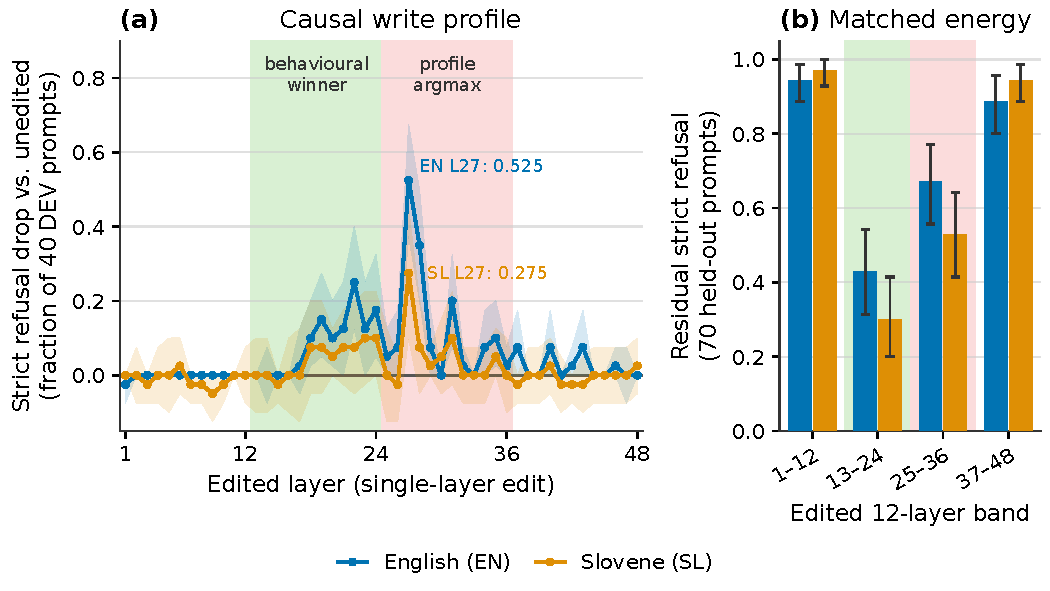
\includegraphics[width=\linewidth,height=0.85\textheight,keepaspectratio]{figures/fig_gams3_profile_v0.pdf}
  \caption{Per-layer refusal drop from single-site ablation in GaMS3. The profile peaks at layer 27 (both EN and SL), in band 25--36, but the behavioural winner at matched energy is band 13--24, the same as in Gemma.}
  \label{fig:gams3_profile}
\end{figure}

\textbf{VERDICT: PARTIAL.} Overlap $O_\mathrm{SL}$ predicts Slovene refusal at Spearman $-$0.900 [$-$0.928, $-$0.857]. \corr{5} Incremental $R^2$ of $O$ over log-energy: 0.580 (LOO: 0.594), passing the 0.10 threshold.

\textbf{Nested $R^2$, GaMS3 SL (each predictor added separately to logE):}

\begin{table}[!htbp]
\centering
\caption{Nested $R^2$, GaMS3 SL (each predictor added separately). Source: \texttt{gen\_art\_experiment\_14}, iteration~4.}
\label{tab:exp14_nested}
\small
\begin{tabular}{lc}
\toprule
Model & $R^2$ \\
\midrule
logE & 0.090 \\
logE + $O$ & 0.669 \\
logE + $O_\mathrm{cos}$ & 0.788 \\
logE + $O_\mathrm{band4}$ & 0.808 \\
logE + $O$ + $O_\mathrm{cos}$ (cumul.) & 0.805 \\
logE + $O$ + $O_\mathrm{cos}$ + $O_\mathrm{band4}$ (cumul.) & 0.822 \\
\bottomrule
\end{tabular}
\end{table}

\textbf{THREE BOUNDARIES:}
\begin{enumerate}
\item $O_\mathrm{band4}$ LOO $\Delta R^2$ = 0.845 and $O_\mathrm{cos}$ = 0.834 both beat $O$'s 0.594: the expensive instrument does not earn its cost over one-forward-pass baselines.
\item The DEV argmax names the wrong band (NAMED\_AND\_LOST).
\item The GaMS3 profile predicts the sibling (Gemma) at Spearman $-$0.442, no worse than its own $-$0.278 on Gemma.
\end{enumerate}

\textbf{Placement vs dose dissociation (A1--A4 ladder).} \corr{5} All four contrasts are Slovene strict. At fixed placement, increasing dose reduces Slovene strict refusal: dose at fixed $O_\mathrm{ship}$ $-$0.186 [$-$0.286, $-$0.086]; dose at fixed $O_\mathrm{swap}$ $-$0.157 [$-$0.257, $-$0.071]. At fixed dose, swapping placement does not significantly change refusal: placement at fixed high E $-$0.029 [$-$0.129, +0.071], McNemar $p$ 0.774; placement at fixed low E +0.000 [$-$0.086, +0.071], $p$ 1.000.

\textbf{Judge certification:} EN $\kappa$ = 0.721 (MISS/JUDGE\_SENSITIVE); SL $\kappa$ = 0.830 (PASS).


\subsection{Experiment 15: Gradient-Blind Fraction}\label{sec:exp15}

\textbf{Goal (gen\_art\_experiment\_15, iteration~4).} Quantify the structural blindness of Heretic's keyword refusal rate.

\textbf{Primary prediction: FALSIFIED.} Paired GBF difference +0.006 [0.000, 0.019]; judge-referenced reverses at $-$0.029.

\begin{table}[!htbp]
\centering
\caption{Keyword objective structural blindness. Source: \texttt{gen\_art\_experiment\_15}, iteration~4.}
\label{tab:exp15_structural}
\small
\begin{tabular}{lcc}
\toprule
& Gemma (anchor) & GaMS3 (sibling) \\
\midrule
Keyword range & [72, 100] & [16, 99] \\
Classifier range & [5, 97] & [0, 98] \\
Slope (keyword on classifier) & 0.308 & 0.738 \\
Mean keyword minus classifier & +20.5 & +15.0 \\
Keyword floor & 72 & 16 \\
GBF (all candidates) & 0.051 & 0.002 \\
GBF (low-C region, C$\leq$50) & 0.470 & 0.017 \\
Threshold blindness fraction (TBF) & 1.0 & 1.0 \\
Self-placebo & 0 & 0 \\
Monotone? & Yes & Yes \\
\bottomrule
\end{tabular}
\end{table}

\begin{figure}[!htbp]
  \centering
  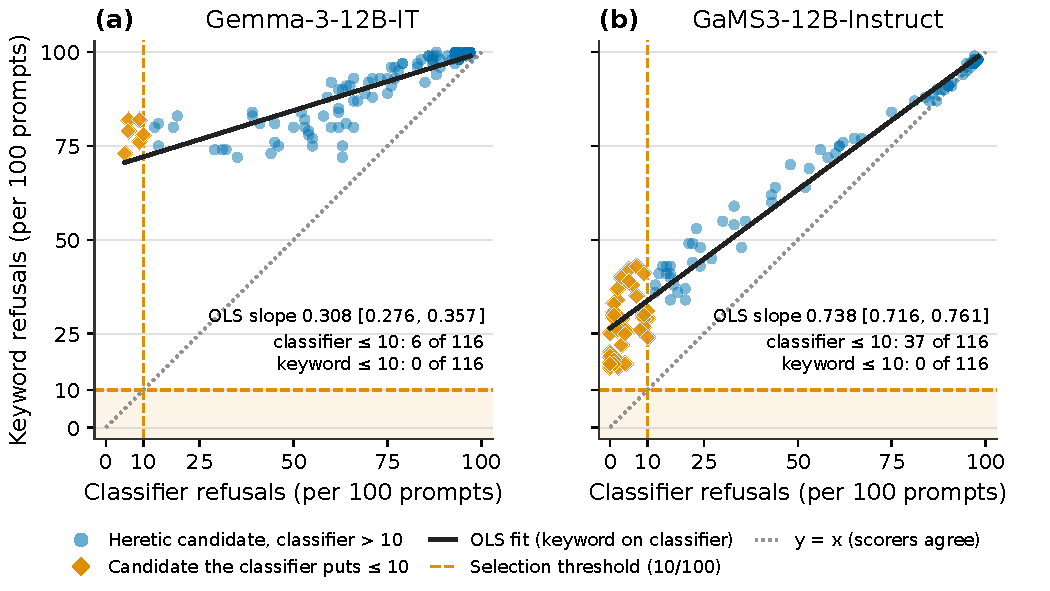
\includegraphics[width=\linewidth,height=0.85\textheight,keepaspectratio]{figures/fig_gbf_v0.pdf}
  \caption{Keyword refusal count vs classifier refusal count across 116 Heretic candidates, for Gemma (left) and GaMS3 (right). The keyword compresses Gemma's range to [72, 100] and never enters the selection threshold region (dashed line at 10).}
  \label{fig:gbf}
\end{figure}

\textbf{Reselection table:}

\begin{table}[!htbp]
\centering
\caption{Reselection under different scorers. Source: \texttt{gen\_art\_experiment\_15}, iteration~4.}
\label{tab:exp15_reselection}
\small
\begin{tabular}{llcl}
\toprule
Model & Scorer & Selected trial & Rule \\
\midrule
Gemma & Keyword (K) & 107 & fallback \\
Gemma & Classifier (C) & 98 & primary \\
Gemma & Qwen3-14B workhorse (J) & 64 & primary \\
GaMS3 & Keyword (K) & 88 & fallback \\
GaMS3 & Classifier (C) & 85 & primary \\
GaMS3 & Qwen3-14B workhorse (J) & 115 & primary \\
\bottomrule
\end{tabular}
\end{table}

\corr{5} The frozen prediction that one search is blinder overall was FALSIFIED. Threshold blindness is shared (TBF = 1.0 in both searches).


\subsection{Evaluation 2: Comprehensive Audit}\label{sec:eval2}

\textbf{Goal (gen\_art\_evaluation\_2, iteration~4).} Audit all prior claims, certify the judge, measure PARTIAL transitions, and quantify the NF4 confound.

\textbf{Judge calibration.} $n$~=~900 items. Overall weighted $\kappa$~=~0.873. Keyword $\kappa$~=~0.074. Classifier $\kappa$~=~0.919. EN gate MET ($\kappa$~0.858). SL gate NOT MET ($\kappa$~0.723).

\textbf{Flip analysis:}

\begin{table}[!htbp]
\centering
\caption{Flip analysis: slope and intercept changes after editing. Source: \texttt{gen\_art\_evaluation\_2}, iteration~4.}
\label{tab:eval2_flip}
\small
\begin{tabular}{llcccc}
\toprule
Model & Lang & Slope ratio [CI] & Intercept & Refit AUROC & Class \\
\midrule
Gemma & EN & 0.50 [0.24, 0.86] & $-$6.65 & $\geq$0.995 & MIXED \\
Gemma & SL & 0.34 [0.19, 0.54] & $-$5.32 & $\geq$0.995 & MIXED \\
GaMS3 & EN & \multicolumn{4}{c}{NOT\_ESTIMABLE (too few refusals after edit)} \\
GaMS3 & SL & \multicolumn{4}{c}{NOT\_ESTIMABLE} \\
\bottomrule
\end{tabular}
\end{table}

\textbf{NF4 vs bf16 confound:} Paired SL--EN strict gap bf16 +0.60 [+0.40, +0.80] vs NF4 +0.45 [+0.20, +0.70], $n$~=~20 S5X pairs, one checkpoint. The difference is not resolved. The asymmetry is at least as large in bf16, so it is not an NF4 artefact.

\textbf{Independent recompute.} 102 numbers checked: 97 match, 3 misdescribed, 2 mismatch. Rate 4.9\% [2.1, 11.0]. All placebos collapse.


\subsection{Research 1: Novelty Positioning}\label{sec:research1}

\textbf{Goal (gen\_art\_research\_1, iteration~4).} Establish what the surviving results add relative to published work.

The surviving positive finding is a matched-total-energy AND matched-layer-count placement contrast. Li et al.~[19] (ICLR 2025) already localise contiguous middle safety layers; Bosco and Srinivasan~[20] locate refusal beyond attention. What this study adds is the energy- and count-matched construction plus the dose rival's failure.

The negative finding---that an activation-space depth measurement fails to predict weight-edit outcomes---positions against Jiang~[21] and AdvPrefix~[22]. \corr{5} AdvPrefix repositioned from the depth result to the selection-blindness companion.


%% ======================================================================
\section{Iteration 5}\label{sec:iter5}

Iteration~5 ran no new experiments; it ran three independent recompute/audit passes and one positioning analysis.


\subsection{Evaluation 3: Terminal Audit}\label{sec:eval3}

\textbf{(gen\_art\_evaluation\_3, iteration~5).} 121 claims checked, 14 discrepancies (11.6\%). 897 assertions classified: 557 OBSERVATION, 285 INTERPRETATION, 45 FAILED\_HYPOTHESIS, 10 UNEXECUTED\_PROPOSAL. No source is a STAND\_IN.


\subsection{Evaluation 4: Report Repairs and Independent Recompute}\label{sec:eval4}

\textbf{(gen\_art\_evaluation\_4, iteration~5).} 136 first-pass numbers recomputed; 21 defective (15.4\%, Wilson 95\% CI [10.3\%, 22.5\%]), of which 14 are material. No number was SIGN\_REVERSED. 8 of 8 placebos collapsed.

\textbf{Citation lint.} 41 file references checked: 27 resolve as written, 14 after rewrite, 0 unresolvable (gate PASS).

\textbf{Failed hypotheses ledger (F1--F17):}

\begin{longtable}{clp{6cm}p{5cm}}
\caption{Evidenced failed hypotheses. Sources: \texttt{gen\_art\_evaluation\_4} (F1--F14) and \texttt{gen\_art\_research\_2} (F15--F17), iteration~5.} \label{tab:dead_ends} \\
\toprule
\# & Status & Hypothesis & What killed it \\
\midrule
\endfirsthead
\toprule
\# & Status & Hypothesis & What killed it \\
\midrule
\endhead
F1 & Killed & Depth coverage explains residual SL refusal over energy & $\Delta R^2$=0.040 but LOO $-$0.002 \\
F2 & Killed & Broad-and-weak beats narrow-and-strong & Falsified opposite: $-$0.10 \\
F3 & Killed & Count-based depth index predicts cross-model residual & Spearman $-$0.009 \\
F4 & Killed & EN/SL direction cosine carries transfer & Spearman +0.010 \\
F5 & Killed & Corrected objective produces a better edit & P7 fired: dose +0.33 vs corrected +0.38 \\
F6 & Killed & Exposure differential carries the surrogacy gap & $\Delta R^2(D|S0) \approx 0$ \\
F7 & Killed & r\_prior direction carries Slovene residual & Cut 0.036 $<$ best random 0.074 \\
F8 & Killed & Thin-margin account explains the gap & Margin-matched gap remains: +0.057 \\
F9 & Killed & Static geometric predictors forecast the gap & CV $R^2 \leq 0$ \\
F10 & Killed & Language-identity direction is a usable lever & FLORES $\Delta$NLL +2.0 \\
F11 & Killed & Depth index EN/SL difference is informative & 4-layer gap inside permutation null \\
F12 & Killed & Energy-matched random ablations are adequate controls & Controls are destructive \\
F13 & Killed & Conformal forecasting is usable & 85\% coverage in only 50\% of cells \\
F14 & Killed & Batched and single generation are interchangeable & B3 certification FAILED \\
F15 & Killed & Effective depth region differs between siblings & DEV band NAMED\_AND\_LOST; placement $p$=0.774 \\
F16 & Killed & Effective region differs by language & Language-label placebo does not collapse: $\rho$ $-$0.94 \\
F17 & Killed & Anchor search is blinder than sibling's & +0.006 [0.000, 0.019]; judge-ref reverses \\
\bottomrule
\end{longtable}

\textbf{Unexecuted proposals (U1--U10):}

\begin{longtable}{clp{5.5cm}p{5.5cm}}
\caption{Unexecuted proposals. Source: \texttt{gen\_art\_evaluation\_4}, iteration~5.} \label{tab:unexecuted} \\
\toprule
\# & & Proposal & Reason \\
\midrule
\endfirsthead
U1 && Native-speaker review of all non-English material & No qualified reviewer; PENDING \\
U2 && Second LLM judge (Gemini) on iter-1 SL arm & Budget block: HTTP 403 \\
U3 && Full gpt-4.1 primary-judge coverage iters 2--3 & Budget block \\
U4 && P2 Sobol sensitivity bands & Cut for time \\
U5 && English-only-vs-full forecast arm & Cut after conformal coverage failure \\
U6 && Language-orthogonalised matched-efficacy arm & Cut for time \\
U7 && EuroLLM-9B-Instruct as M3 & Gated repository, HTTP 403 \\
U8 && Racing placement against published cheap predictors & Identified only in positioning; not run \\
U9 && Iter-1 experiment pods 2 and 4 & Empty workspaces \\
U10 && Iteration-4 arms not reached & See per-pod deviations \\
\bottomrule
\end{longtable}


\subsection{Evaluation 5: Keyword Blindness Decomposition}\label{sec:eval5}

\textbf{(gen\_art\_evaluation\_5, iteration~5).} Decomposed the keyword objective's blindness into per-language components on verified translation pairs.

\textbf{Held-out agreement per language.} On edited English outputs, keyword $\kappa$~=~0.021 ($n$=490). It misfires: calls 0.341 of responses refusals where the reference sees 0.173, and 0.814 of its ``refusals'' are false. On edited Slovene outputs $\kappa$~=~0.000: the rule is SILENT and fires on 0 of 490 responses, while the reference sees refusal in 0.439.

\textbf{Cross-lingual measurement bias.} On the 100 verified EN--SL pairs for the main Gemma edit, keyword score discrepancy from the workhorse judge: $d_\mathrm{EN}$~=~+0.74 and $d_\mathrm{SL}$~=~$-$0.82, so $\Delta_\mathrm{lang}$~=~$-$1.56 [$-$1.68, $-$1.44]. In Slovene all discrepancy is missed refusals (FN rate 0.82, FP rate 0.00). In English the rule over-reports (FP rate 0.78). Disagreement RATES happen to be equal (McNemar $p$~=~1.00), but DIRECTIONS differ (sign test $p$~=~5.0e-29).

\textbf{Judge sensitivity.} Registry counts: JUDGE\_ROBUST 6, JUDGE\_SENSITIVE 72.


\subsection{Research 2: Positioning Against Nearest Published Work}\label{sec:research2}

\textbf{(gen\_art\_research\_2, iteration~5).} Positioned the surviving results against neighbours.

\textbf{Qualifiers checked:}
\begin{itemize}
\item Selection of sites by measured causal effect: DROPPED (covered by [26], [21]).
\item Depth-localised vs distributed refusal: DROPPED (covered by [23], [24]).
\item Layer sensitivity differs per language: NARROWED (covered by [25]; claim is only the edit-placement consequence).
\item Failed dose rival at matched placement: KEPT.
\item Outside-family replication (Qwen3-8B): KEPT.
\item Matched total edit size AND matched layer count: KEPT, NARROWED.
\item Effective region differs between sibling checkpoints: DROPPED (FALSIFIED by F15).
\end{itemize}

\textbf{Bibliography repairs.} [19] venue year corrected (ICLR 2025, not 2024); arXiv IDs added for [20] and [21]. AdvPrefix [22] repositioned from depth result to selection-blindness companion.


%% ======================================================================
\section{What We Have Learned}\label{sec:learned}

\begin{figure}[!htbp]
  \centering
  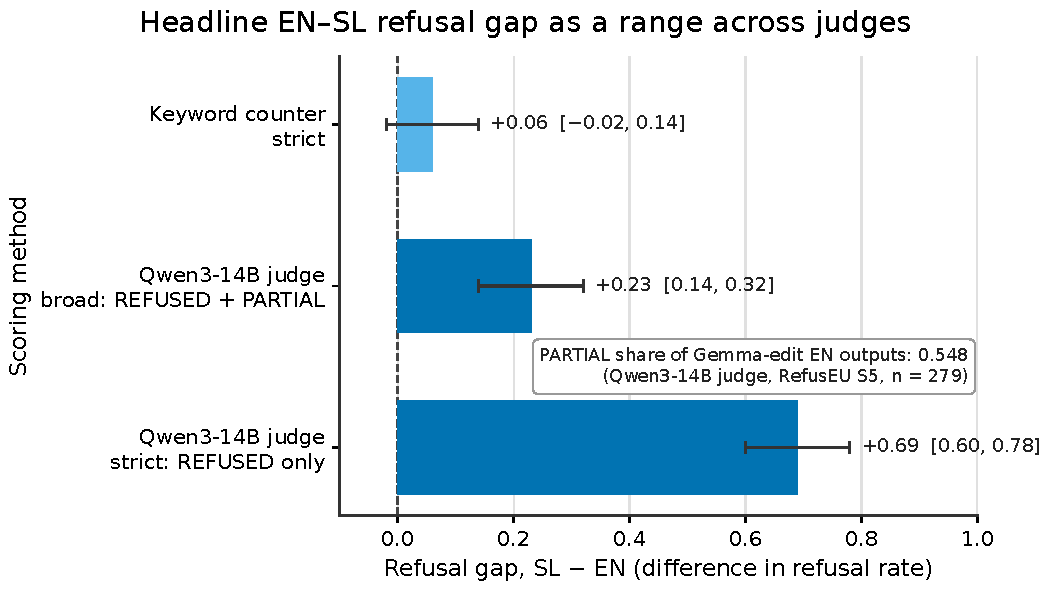
\includegraphics[width=\linewidth,height=0.85\textheight,keepaspectratio]{figures/fig_refusal_gap_v0.pdf}
  \caption{The Gemma edit S5X paired EN--SL refusal gap under three scoring methods. The gap ranges from +0.06 (keyword strict) to +0.69 (Qwen3-14B strict); the PARTIAL class is the wedge.}
  \label{fig:refusal_gap}
\end{figure}

Five iterations have converged on a picture with one firm positive, one transferable negative, a structural measurement finding, and seventeen falsified predictions.

\textbf{Firm positive: matched-budget placement orders residual refusal.} At matched total removal energy AND matched layer count, where in depth an English-derived refusal edit deposits that energy orders how much refusal survives: in both languages, in two sibling checkpoints, and in an outside family (Qwen3-8B), and not recoverable by doubling the dose of a badly placed edit. The band is shared; the residual is not. The English causal write profile predicts the Slovene residual at $\rho$ $-$0.94, so the language-label placebo does not collapse; what differs by language is how much refusal is left at the same placement and energy (strict refusal EN 0.07 vs SL 0.27 in group G3). Two one-forward-pass baselines ($O_\mathrm{cos}$ and $O_\mathrm{band4}$) match or beat the expensive single-layer causal instrument. At the refusal floor of shipped edits, dose not placement is the active variable ($p$~0.774 / 1.000).

\textbf{Transferable negative: the activation-space depth index fails to predict weight-edit outcomes.} Spearman $-$0.009 over 21 rows (comparing Gemma with Qwen3-8B, plus excluded Mistral). The EN/SL direction cosine fails beside it (Spearman +0.010). Two baselines beat both: single-site causal transfer rate +0.732 and unedited model's own refusal rate +0.661.

\textbf{Structural measurement finding: the keyword objective is cross-lingually biased.} On verified translation pairs, $\Delta_\mathrm{lang}$~=~$-$1.56 [$-$1.68, $-$1.44]: the English keyword rule over-reports in English (FP rate 0.78) and is silent in Slovene (FN rate 0.82). Threshold blindness is 1.0 in both searches. The pre-registered prediction that one search is blinder overall was FALSIFIED.

\textbf{Seventeen hypotheses falsified} across five iterations (F1--F17): depth coverage (F1), broad-beats-narrow (F2), count-based cross-model index (F3), direction cosine (F4), corrected objective (F5), exposure differential (F6), r\_prior (F7), thin-margin (F8), static geometry (F9), language-identity lever (F10), depth index difference (F11), random controls (F12), conformal forecasting (F13), batch interchangeability (F14), sibling band difference (F15), language band difference (F16), and anchor blinder (F17).

\textbf{The headline gap stated as a range.} The Gemma edit S5X paired EN--SL gap ranges from +0.06 (keyword strict) to +0.69 (Qwen3-14B strict), with the broad definition at +0.23. On GaMS3, all judges agree the gap is near zero. The PARTIAL class (0.548 of Gemma edit EN outputs) is the wedge. The Slovene judge certification gate was not met ($\kappa$ 0.723 $<$ 0.80), so all Slovene gap claims remain judge-sensitive. 94--95\% of edited English outputs were truncated at the 256-token generation cap.

\textbf{Scope and limits.} Two sibling checkpoints of one architecture plus one outside family; one non-English language in the matched panels (two further languages only in the outside-family arm); one or two optimiser seeds; NF4 throughout with a single bf16 control cell (paired SL--EN gap bf16 +0.60 [+0.40, +0.80] vs NF4 +0.45 [+0.20, +0.70], not resolved but the asymmetry is at least as large in bf16); Slovene material machine-translated with native review PENDING. Two checkpoints are two units, not a population: nothing is attributed to Slovene continual pretraining, instruction tuning, or any safety-training stage. Five packets totalling 640 items remain pending for native-speaker labelling. Every judged rate in the report is proxy-certified, not human-certified. 136 numbers independently re-derived in iteration~5; defect rate 15.4\% [10.3\%, 22.5\%] on previously unaudited sections.


%% ======================================================================
\section{Run Trajectory}\label{sec:trajectory}

\begin{table}[!htbp]
\centering
\caption{Run trajectory: one row per iteration. ``Ledger spend'' is cumulative LLM/tool/container spend billed through that iteration; it excludes compute-rental time and is not the run's total cost.}
\label{tab:trajectory}
\small
\begin{tabular}{cllclc}
\toprule
Iter & Hypothesis & Move & Score & Executed & Ledger (\$) \\
\midrule
1 & What EN abliteration misses in SL & --- & --- & Yes & 6.07 \\
2 & SL refusal needs a deeper edit & deepen & 3 & Yes & 42.31 \\
3 & Where the edit lands, not how deep & deepen & 4 & Yes & 161.91 \\
4 & Where the edit lands beats how hard & deepen & 3 & Yes & 258.92 \\
5 & Where the edit lands beats how hard & deepen & 3 & Yes & 270.89 \\
\bottomrule
\end{tabular}
\end{table}


%% ======================================================================
\section{References}\label{sec:references}

\begin{enumerate}
\item[{[1]}] Arditi, A.\ et al.\ (2024). Refusal in Language Models Is Mediated by a Single Direction. arXiv:2406.11717.
\item[{[2]}] Wang, X.\ et al.\ (2025). Refusal Direction is Universal Across Safety-Aligned Languages. arXiv:2505.17306.
\item[{[3]}] Krasnodebska, A., Kusa, W., and Lipani, A.\ (2026). Multilingual Refusal Alignment for Safer Large Language Models. ACL 2026 Findings. arXiv:2606.07535.
\item[{[4]}] Stein, E.~V.\ et al.\ (2026). BabelSteering: Multilingual Safety Alignment via English Steering Vectors. arXiv:2608.16577.
\item[{[5]}] Yoon, C., Park, J., and Ritter, A.\ (2026). Who Pays More for Safety? EMNLP 2026. arXiv:2608.22490.
\item[{[6]}] Aziz, R., Hanif, I.~A., and Koto, F.\ (2026). Low-Resource Safety Failures Are Action Failures, Not Representation Failures. arXiv:2606.01196.
\item[{[7]}] Wu, J.\ et al.\ (2026). Knowing without Acting: The Disentangled Geometry of Safety Mechanisms in LLMs. arXiv:2603.05773.
\item[{[8]}] Fafula, A.\ (2026). Abliteration Is Not a Scalpel. arXiv:2607.17427.
\item[{[9]}] Upadhyaya, A.\ and Sikdar, S.\ (2026). When Safety Speaks a Language. arXiv:2608.29936.
\item[{[10]}] Hawkins, W.\ et al.\ (2026). The Heterogeneous Safety Impacts of Benign Multilingual Fine-Tuning. arXiv:2606.28843.
\item[{[11]}] Labunets, A.\ (2026). Refusal geometry reflects refusal training. arXiv:2608.25390.
\item[{[12]}] Marchisio, K.\ et al.\ (2024). How Does Quantization Affect Multilingual LLMs? EMNLP 2024. arXiv:2407.03211.
\item[{[13]}] Chimoto, E., Elhoushi, M., and Bassett, B.\ (2026). Calibrating Beyond English. EACL 2026. arXiv:2601.18306.
\item[{[14]}] Young, R.\ (2025). Comparative Analysis of LLM Abliteration Methods. arXiv:2512.13655.
\item[{[15]}] Petrov, V.\ (2026). On the Failure of Topic-Matched Contrast Baselines. arXiv:2603.22061.
\item[{[16]}] Tang, T.\ et al.\ (2024). Language-Specific Neurons. ACL 2024. arXiv:2402.16438.
\item[{[17]}] Ghussin, Y.\ et al.\ (2026). Multilingual Steering by Design. TrustNLP 2026. arXiv:2605.23036.
\item[{[18]}] Frank, G.~N.\ (2026). Detection Is Cheap, Routing Is Learned. arXiv:2603.18280.
\item[{[19]}] Li, S.\ et al.\ (2025). Safety Layers in Aligned Large Language Models. ICLR 2025. arXiv:2408.17003.
\item[{[20]}] Bosco, P.~C.\ and Srinivasan, G.\ (2026). Locating and Steering Refusal Beyond Attention. arXiv:2609.04721.
\item[{[21]}] Jiang, Y.\ (2026). Refit the Probe: Single-Direction Ablation Is Not a Necessity Test. arXiv:2606.00926.
\item[{[22]}] Zhu, S.\ et al.\ (2025). AdvPrefix: An Objective for Nuanced LLM Jailbreaks. arXiv:2412.10321.
\item[{[23]}] Hadetskyi, O.\ (2026). Abliteration Unleashed. arXiv:2607.02714.
\item[{[24]}] Zong, Y.\ et al.\ (2026). Localizing Safety-Critical Layers in LLMs by Transplanting Refusal Behaviour. arXiv:2608.11583.
\item[{[25]}] Li, W.\ et al.\ (2026). Safety-Sensitive Layers Are Not Monolingual. arXiv:2609.22144.
\item[{[26]}] Wang, Z.\ et al.\ (2026). Probe-Best Is Not Steer-Best. arXiv:2609.22135.
\item[{[27]}] Agnihotri, S., Khandelwal, A., and Bansal, M.\ (2025). Abliteration Has Limits. NeurIPS 2025 Workshop. arXiv:2510.02768.
\item[{[28]}] Schwinn, L.\ et al.\ (2026). How Reliable Are LLM-as-a-Judge in Red-Teaming Evaluation? arXiv:2603.06594.
\item[{[29]}] Zhang, Y.\ et al.\ (2026). Multilingual Safety Judge for LLMs. COLM 2026. arXiv:2605.17173.
\item[{[30]}] Kurz, S.\ et al.\ (2026). On the Limitations of Language-targeted Pruning. TACL vol.~14, pp.~167--192. arXiv:2408.14398.
\end{enumerate}

\end{document}
